\documentclass[12pt,a4paper]{report}

\usepackage{graphicx}
\usepackage{setspace}
\usepackage{geometry}
\usepackage{parskip}
\usepackage{float}
\usepackage{array}
\usepackage{tabularx}
\usepackage{listings}
\usepackage{placeins}
\usepackage{rotating}
\geometry{left=1in, right=1in, top=1in, bottom=1in}
\graphicspath{{images/}}

% Let figures share pages with text and pack float pages more fully, so a short
% figure does not sit alone on an otherwise blank page.
\renewcommand{\topfraction}{0.9}
\renewcommand{\bottomfraction}{0.8}
\renewcommand{\textfraction}{0.07}
\renewcommand{\floatpagefraction}{0.7}
\setcounter{topnumber}{3}
\setcounter{bottomnumber}{2}
\setcounter{totalnumber}{4}

% Clean, black-and-white monospace style for the occasional code listing.
\lstset{
  basicstyle=\ttfamily\small,
  breaklines=true,
  columns=flexible,
  keepspaces=true,
  showstringspaces=false,
  frame=single,
  framesep=4pt,
  xleftmargin=1em,
  aboveskip=1em,
  belowskip=1em
}

\begin{document}
\begin{titlepage}
    \centering

    % Institute
    {\Large\bfseries COEP Technological University, Pune}\par
    \vspace{0.4cm}

    % Department
    {\Large Department of Computer Science and Engineering}\par
    \vspace{1.8cm}

    % Title
    {\Huge\bfseries INTERNSHIP REPORT}\par
    \vspace{0.6cm}

    \begin{figure}[H]
        \centering
        
\includegraphics[width=0.35\linewidth]{coep_logo.png}
        \label{fig:logo}
    \end{figure}

    % Internship info
    \begin{spacing}{1.2}
        \Large
        \begin{tabular}{rl}
            \textbf{Internship Duration:} & 03/06/2026 -- 29/07/2026\\[8pt]
            \textbf{Academic Year:} & Final Year BTech 2026--27\\
        \end{tabular}
    \end{spacing}

    \vspace{1.6cm}

    % Submitted by
    {\Large\textbf{Submitted by}}\par
    \vspace{0.35cm}
    {\Large \textbf{Chaithanya Gopi Hosahudya}}\par
    \vspace{0.15cm}
    {\large MIS: \textbf{612303041}}\par

    \vspace{1.6cm}

    % Mentors
    \begin{spacing}{1.3}
        \Large
        \textbf{Internal Mentor:} Dr.\ Pratiksha Deshmukh\\[10pt]
        \textbf{External Mentor:} Neela Santhosh Kumar, Human Resources \& Academic Head, CodTech IT Solutions Pvt.\ Ltd.
    \end{spacing}

    \vfill
    {\small \today}
\end{titlepage}
\tableofcontents

\chapter*{Introduction}
\addcontentsline{toc}{chapter}{Introduction}

Competitive programming judges, often called online judges, are systems that accept a program written by a user, run it against a fixed set of test cases and decide automatically whether the program is correct and efficient enough. They are the backbone of programming contests and practice sites, where a single problem may receive thousands of submissions in many different languages. Each submission must be compiled, executed under strict time and memory limits and compared against the expected output, and all of this must happen quickly and fairly so that two users who submit the same solution always receive the same result.

Building such a system is harder than it first appears, because the code being executed is untrusted. A judge must run programs written by complete strangers on its own machines, and some of those programs may be buggy, badly behaved or deliberately malicious. A submission might try to read other users' data, open network connections, consume all available memory, spawn an unbounded number of processes or simply loop forever. The judge therefore has to isolate every submission from the host and from every other submission, place hard limits on the resources it may use and guarantee that a single bad program cannot affect the stability of the service or the correctness of anyone else's result. Fairness adds a further requirement, as the same program must be measured under the same conditions every time it runs.

The internship project described in this report was the design and implementation of a complete competitive programming platform that addresses these concerns. The system consists of a React single page application for the user interface, a Spring Boot backend that exposes a REST API and a judge engine that executes each submission inside an isolated, resource limited Docker container. The platform supports user registration and login with JSON Web Tokens, administrator managed problems with public and hidden test cases, submission and judging in C++, Java and Python, a range of verdicts such as Accepted, Wrong Answer, Time Limit Exceeded and Compile Error, and a leaderboard backed by Redis. Particular attention was given to running untrusted code safely, to keeping the judging process robust under failure and to keeping the database transactions short so that the system behaves well under load.

This report begins with the objectives of the internship and a short description of the host organisation, followed by the scope of the work. The main chapter, Activities Undertaken, follows the sequence of work recorded in the internship timesheet, moving from the initial learning phase through system design, authentication, the judge engine, the leaderboard, the frontend, containerisation and testing. The later chapters reflect on the skills gained, the challenges faced, the impact of the work, and recommendations for how the platform could be extended in the future.

\chapter*{Objectives}
\addcontentsline{toc}{chapter}{Objectives}

The main objectives of the internship were as follows:

\begin{itemize}
    \item To design and build a full stack competitive programming platform with a Spring Boot backend, a React frontend and a PostgreSQL database, applying the concepts studied during the learning phase to a realistic project.

    \item To implement secure, stateless authentication and authorisation using JSON Web Tokens, BCrypt password hashing and role based access control for ordinary users and administrators.

    \item To build a judge engine that compiles and runs untrusted submissions in C++, Java and Python inside isolated, resource limited Docker containers, and to assign the correct verdict to each submission.

    \item To make the judging process robust by enforcing time, memory and output limits, cleaning up containers and workspaces reliably and keeping database transactions short so that the system scales well.

    \item To implement a leaderboard using a Redis sorted set as a cache over PostgreSQL, together with per user submission rate limiting and consistent error handling.

    \item To develop a clear and usable frontend with a code editor, problem pages, a submission status page and a leaderboard, and to package the whole system with Docker Compose for easy deployment.

    \item To validate the platform through automated unit and integration tests and an end to end smoke test covering all three languages, and to document the design and the reasoning behind it.
\end{itemize}

\chapter*{About the Organization}
\addcontentsline{toc}{chapter}{About the Organization}

% TODO: verify organisation details
This internship was carried out at CodTech IT Solutions Pvt.\ Ltd., an information technology services company that works in the area of software development and provides structured internship programmes for students. The organisation offers practical, project based training in which interns work on software development tasks under the guidance of an industry mentor, with the aim of bridging the gap between academic study and professional engineering practice.

The internship programme is designed to give students exposure to the full software development process, from understanding requirements and designing a system to implementing, testing and documenting it. Interns are encouraged to use current tools and frameworks, to follow good engineering practices and to take ownership of a complete piece of work rather than a small isolated task. This approach suited the present project well, since building a competitive programming platform required designing and implementing a complete system spanning the frontend, the backend, the database and the execution environment.

The work in this report was carried out under the external mentorship of Neela Santhosh Kumar, Human Resources \& Academic Head at CodTech IT Solutions, who provided direction on the project requirements, and under the internal guidance of Dr.\ Pratiksha Deshmukh from COEP Technological University. The combination of an industry defined project and academic supervision provided a useful setting for applying theoretical knowledge to a practical software engineering problem.

\chapter*{Scope of Work}
\addcontentsline{toc}{chapter}{Scope of Work}

The scope of the internship was to design and build a complete competitive programming platform and to make it robust enough to serve as a realistic demonstration of an online judge. The work covered every layer of the system, beginning with the backend, which was implemented as a Spring Boot application exposing a REST API for authentication, problem management, submission handling and the leaderboard. The backend was organised into controllers, services, repositories and entities, with the judging logic kept in its own group of classes so that it could be reasoned about and tested independently.

A central part of the scope was the judge engine, which is responsible for compiling and executing untrusted submissions and deciding their verdicts. This required designing a per submission workspace, invoking a separate sandbox for the compile step and for each test case, comparing program output against the expected output and distinguishing between the various failure modes such as wrong answer, time limit exceeded, memory limit exceeded, output limit exceeded, runtime error and compile error. Closely related to this was the sandboxing work, in which small runner images were built for each language and every execution was confined using the isolation and resource control features of Docker.

The scope also included the frontend, built as a React single page application with a Monaco based code editor, pages for browsing and viewing problems, a submission status page that polls for the verdict and a leaderboard page, along with the authentication context that manages the user's tokens. Supporting these were the cross cutting concerns of asynchronous submission processing, per user rate limiting, input validation and consistent error responses. Finally, the scope covered deployment and testing: packaging the whole system with Docker Compose, and validating it through unit tests, an integration test of the authentication flow and an end to end smoke test exercising all three languages across the full range of verdicts.

\chapter*{Activities Undertaken}
\addcontentsline{toc}{chapter}{Activities Undertaken}

\section*{Learning Phase}
The internship began with a structured learning phase to build the foundation needed for the project. The first part was a revision of core Java, covering object oriented concepts such as classes, inheritance, polymorphism and interfaces, followed by the collections framework, exception handling, generics and file input and output. The more recent features of the language were also revised, including lambda expressions, functional interfaces, the Streams API and the concurrency utilities such as the executor service, since these would later be relevant to asynchronous processing in the judge.

The focus then moved to the Spring ecosystem, which forms the core of the backend. Time was spent understanding the Spring Boot project structure, the Maven build, starters and the use of the application configuration file. The central ideas of the Spring container, namely inversion of control and dependency injection, were studied along with the annotations used to declare beans and wire them together. Building on this, REST API development with Spring MVC was practised using controllers, request mappings and data transfer objects, and persistence was studied through Spring Data JPA and Hibernate, including entity relationships, repositories and pagination, with the application connected to a PostgreSQL database.

The final part of the learning phase covered the topics most specific to this project. Spring Security was studied with a focus on authentication, authorisation and password hashing with BCrypt, followed by stateless authentication using JSON Web Tokens with separate access and refresh tokens. Docker was learned from first principles, covering images, containers, the Dockerfile and Docker Compose, since the judge depends heavily on containerisation. Asynchronous processing with the Spring {\ttfamily @Async} annotation was also studied, and a small practice application was built to tie these ideas together before the main project began.

\section*{Requirement Analysis and System Architecture}
With the learning phase complete, the project began with a short requirement analysis and the design of the overall architecture. The platform needed to allow users to register and log in, browse problems, submit solutions in several languages and view their verdicts, while administrators needed to be able to create and manage problems. Underlying all of this was the firm requirement that user submitted code must be executed safely and fairly, which shaped many later decisions.

The architecture that emerged is a single Spring Boot application, or monolith, backed by PostgreSQL for persistent data and Redis for the leaderboard, with a React frontend served through nginx. A monolithic design was chosen deliberately because it is simpler to build, deploy and reason about at this scale, while the judging logic was kept in its own self contained group of classes so that it could be extracted into a separate service later if horizontal scaling were ever required. The backend launches a fresh, isolated Docker container for every compile step and every test case, using the host Docker daemon. Figure~\ref{fig:architecture} shows the overall structure and the main flow of requests through the system.

\begin{figure}[htbp]
  \centering
  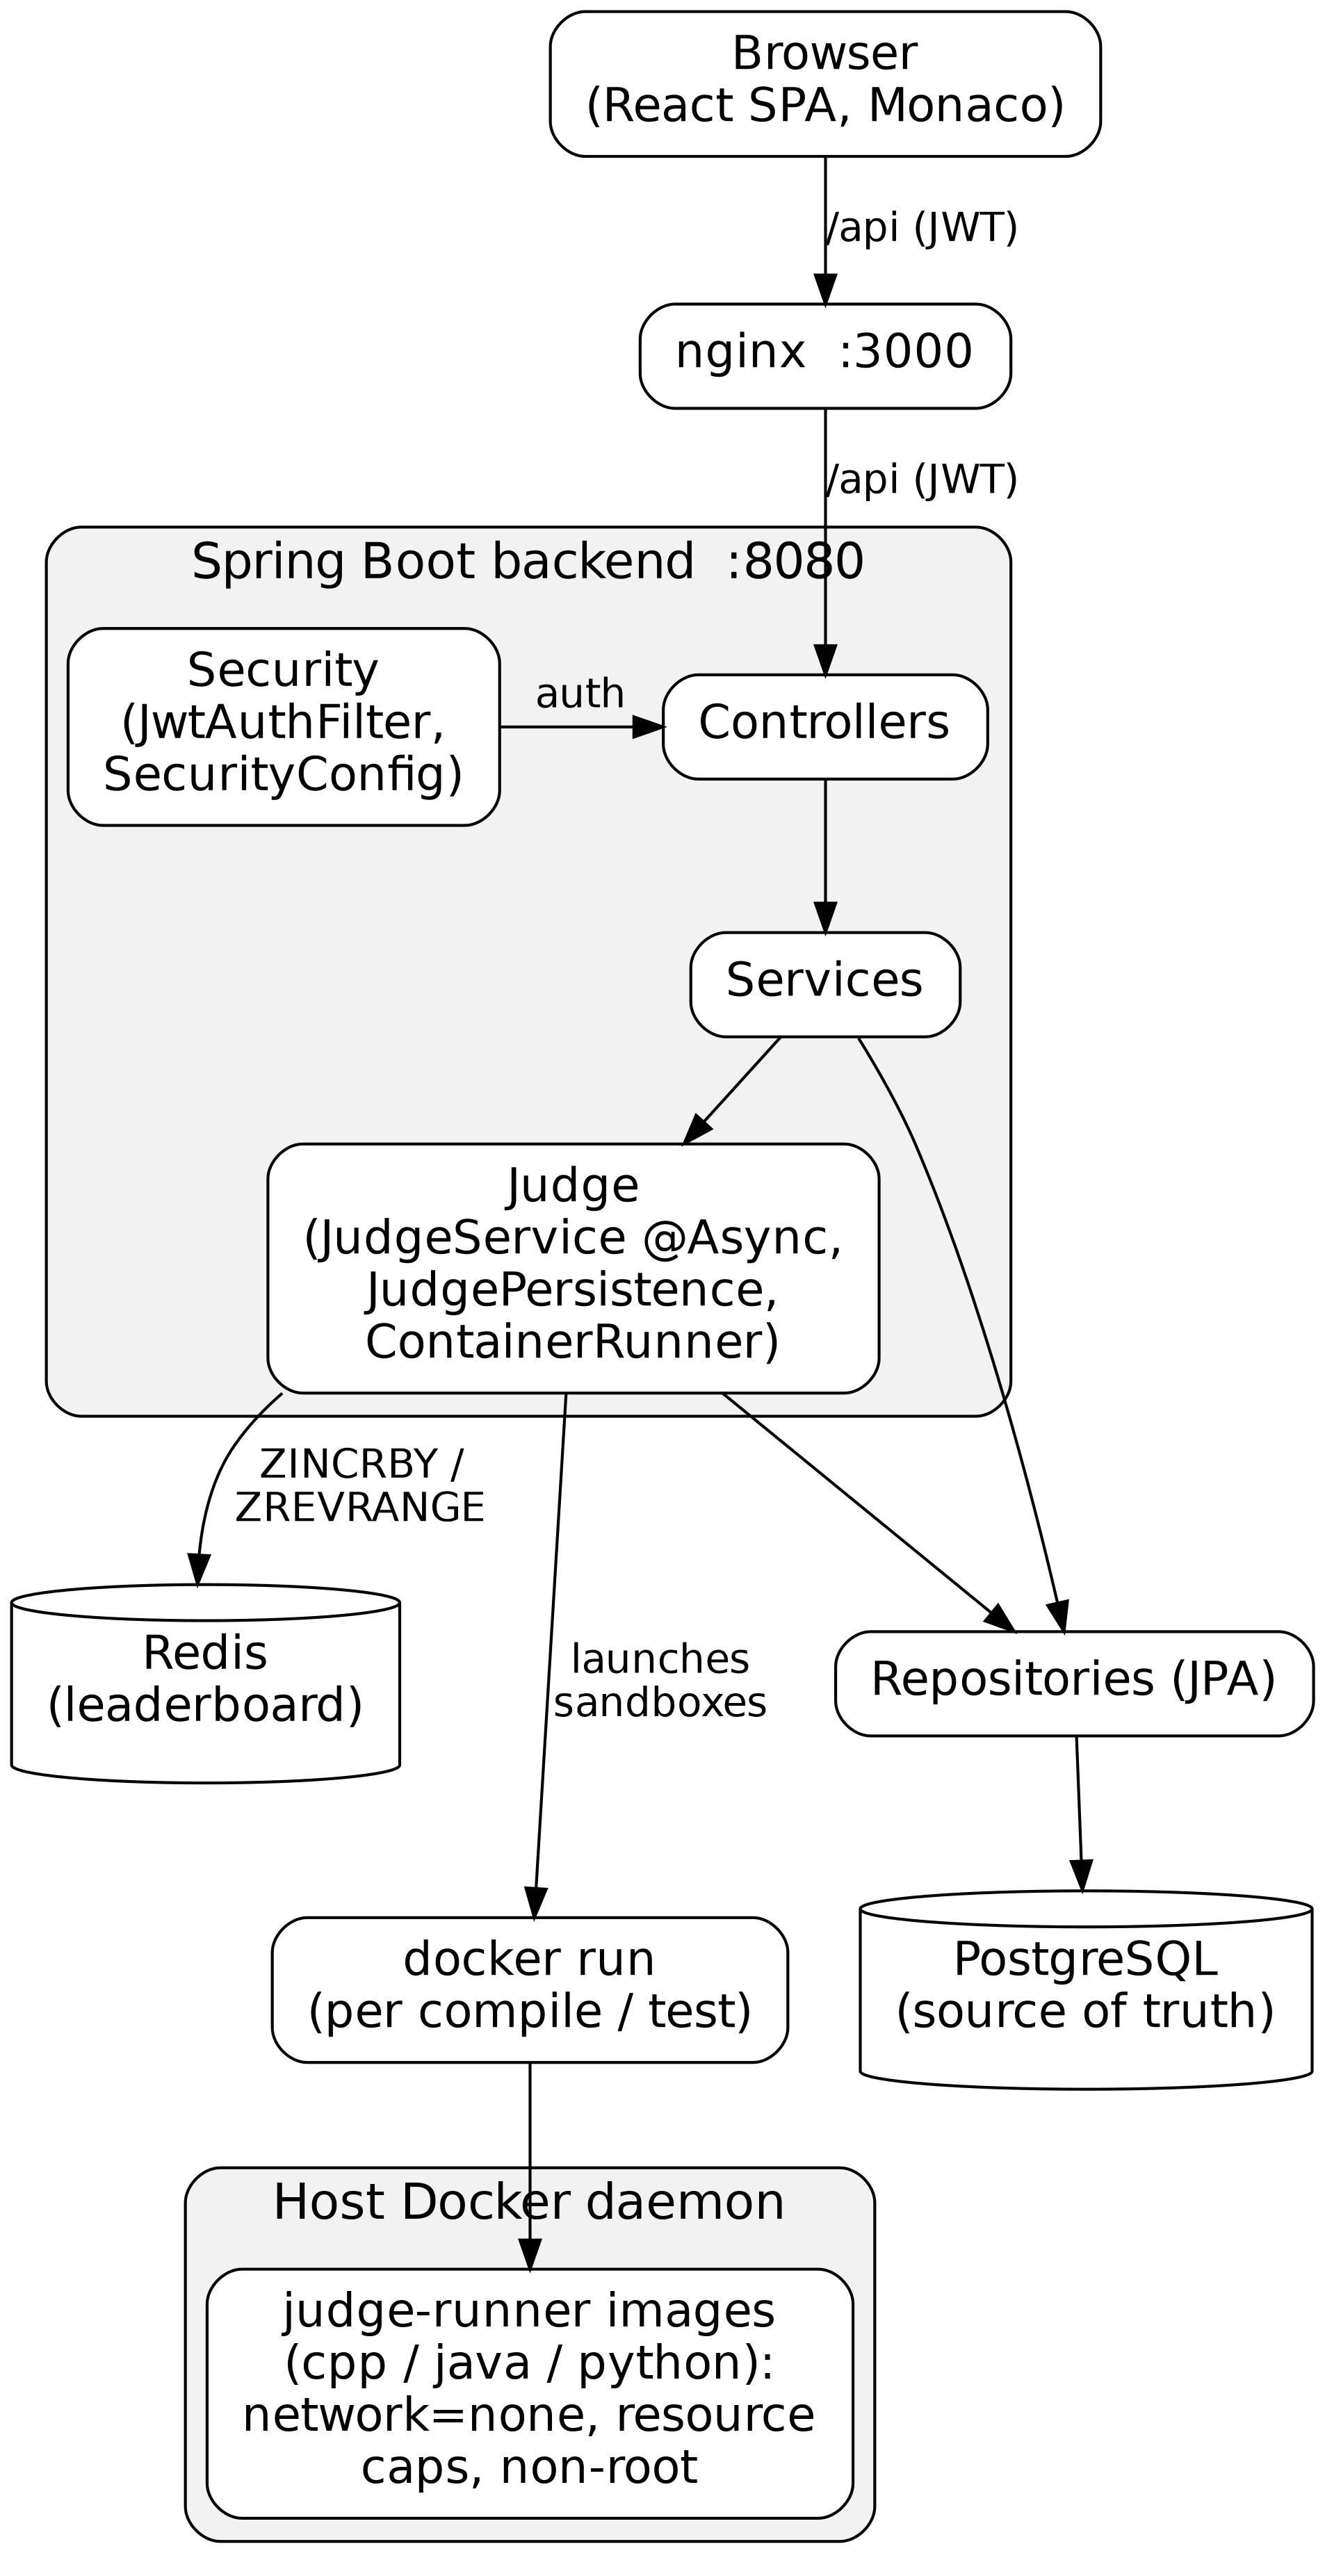
\includegraphics[width=0.68\textwidth]{architecture.png}
  \caption{High level architecture of the platform, showing the React frontend, the layered Spring Boot backend, the PostgreSQL and Redis data stores, and the sandbox containers launched on the host Docker daemon.}
  \label{fig:architecture}
\end{figure}

\section*{Database Design}
The next activity was the design of the database schema, which was implemented as a set of JPA entities mapped to PostgreSQL tables. The central entity is the User, which holds the email, username, BCrypt password hash and a role that is either an ordinary user or an administrator. Problems are represented by the Problem entity, which carries the title, a unique slug, a difficulty, the statement, and the time and memory limits; each problem has a set of Tag entities through a many to many relationship and a collection of TestCase entities, each of which may be marked public or hidden.

Submissions and their outcomes are modelled by three further entities. A Submission records the user, the problem, the language, the source code, the overall status and score, and timestamps. Each run of a submission against a single test case produces a SubmissionResult, which stores the per test verdict and runtime, so that the submission page can show a breakdown across all test cases. Finally, a UserProgress entity records, for each user and problem pair, whether the problem has been solved and how many attempts have been made, which is the information the leaderboard is built from. The relationships between these entities are shown in Figure~\ref{fig:er}.

\begin{sidewaysfigure}
  \centering
  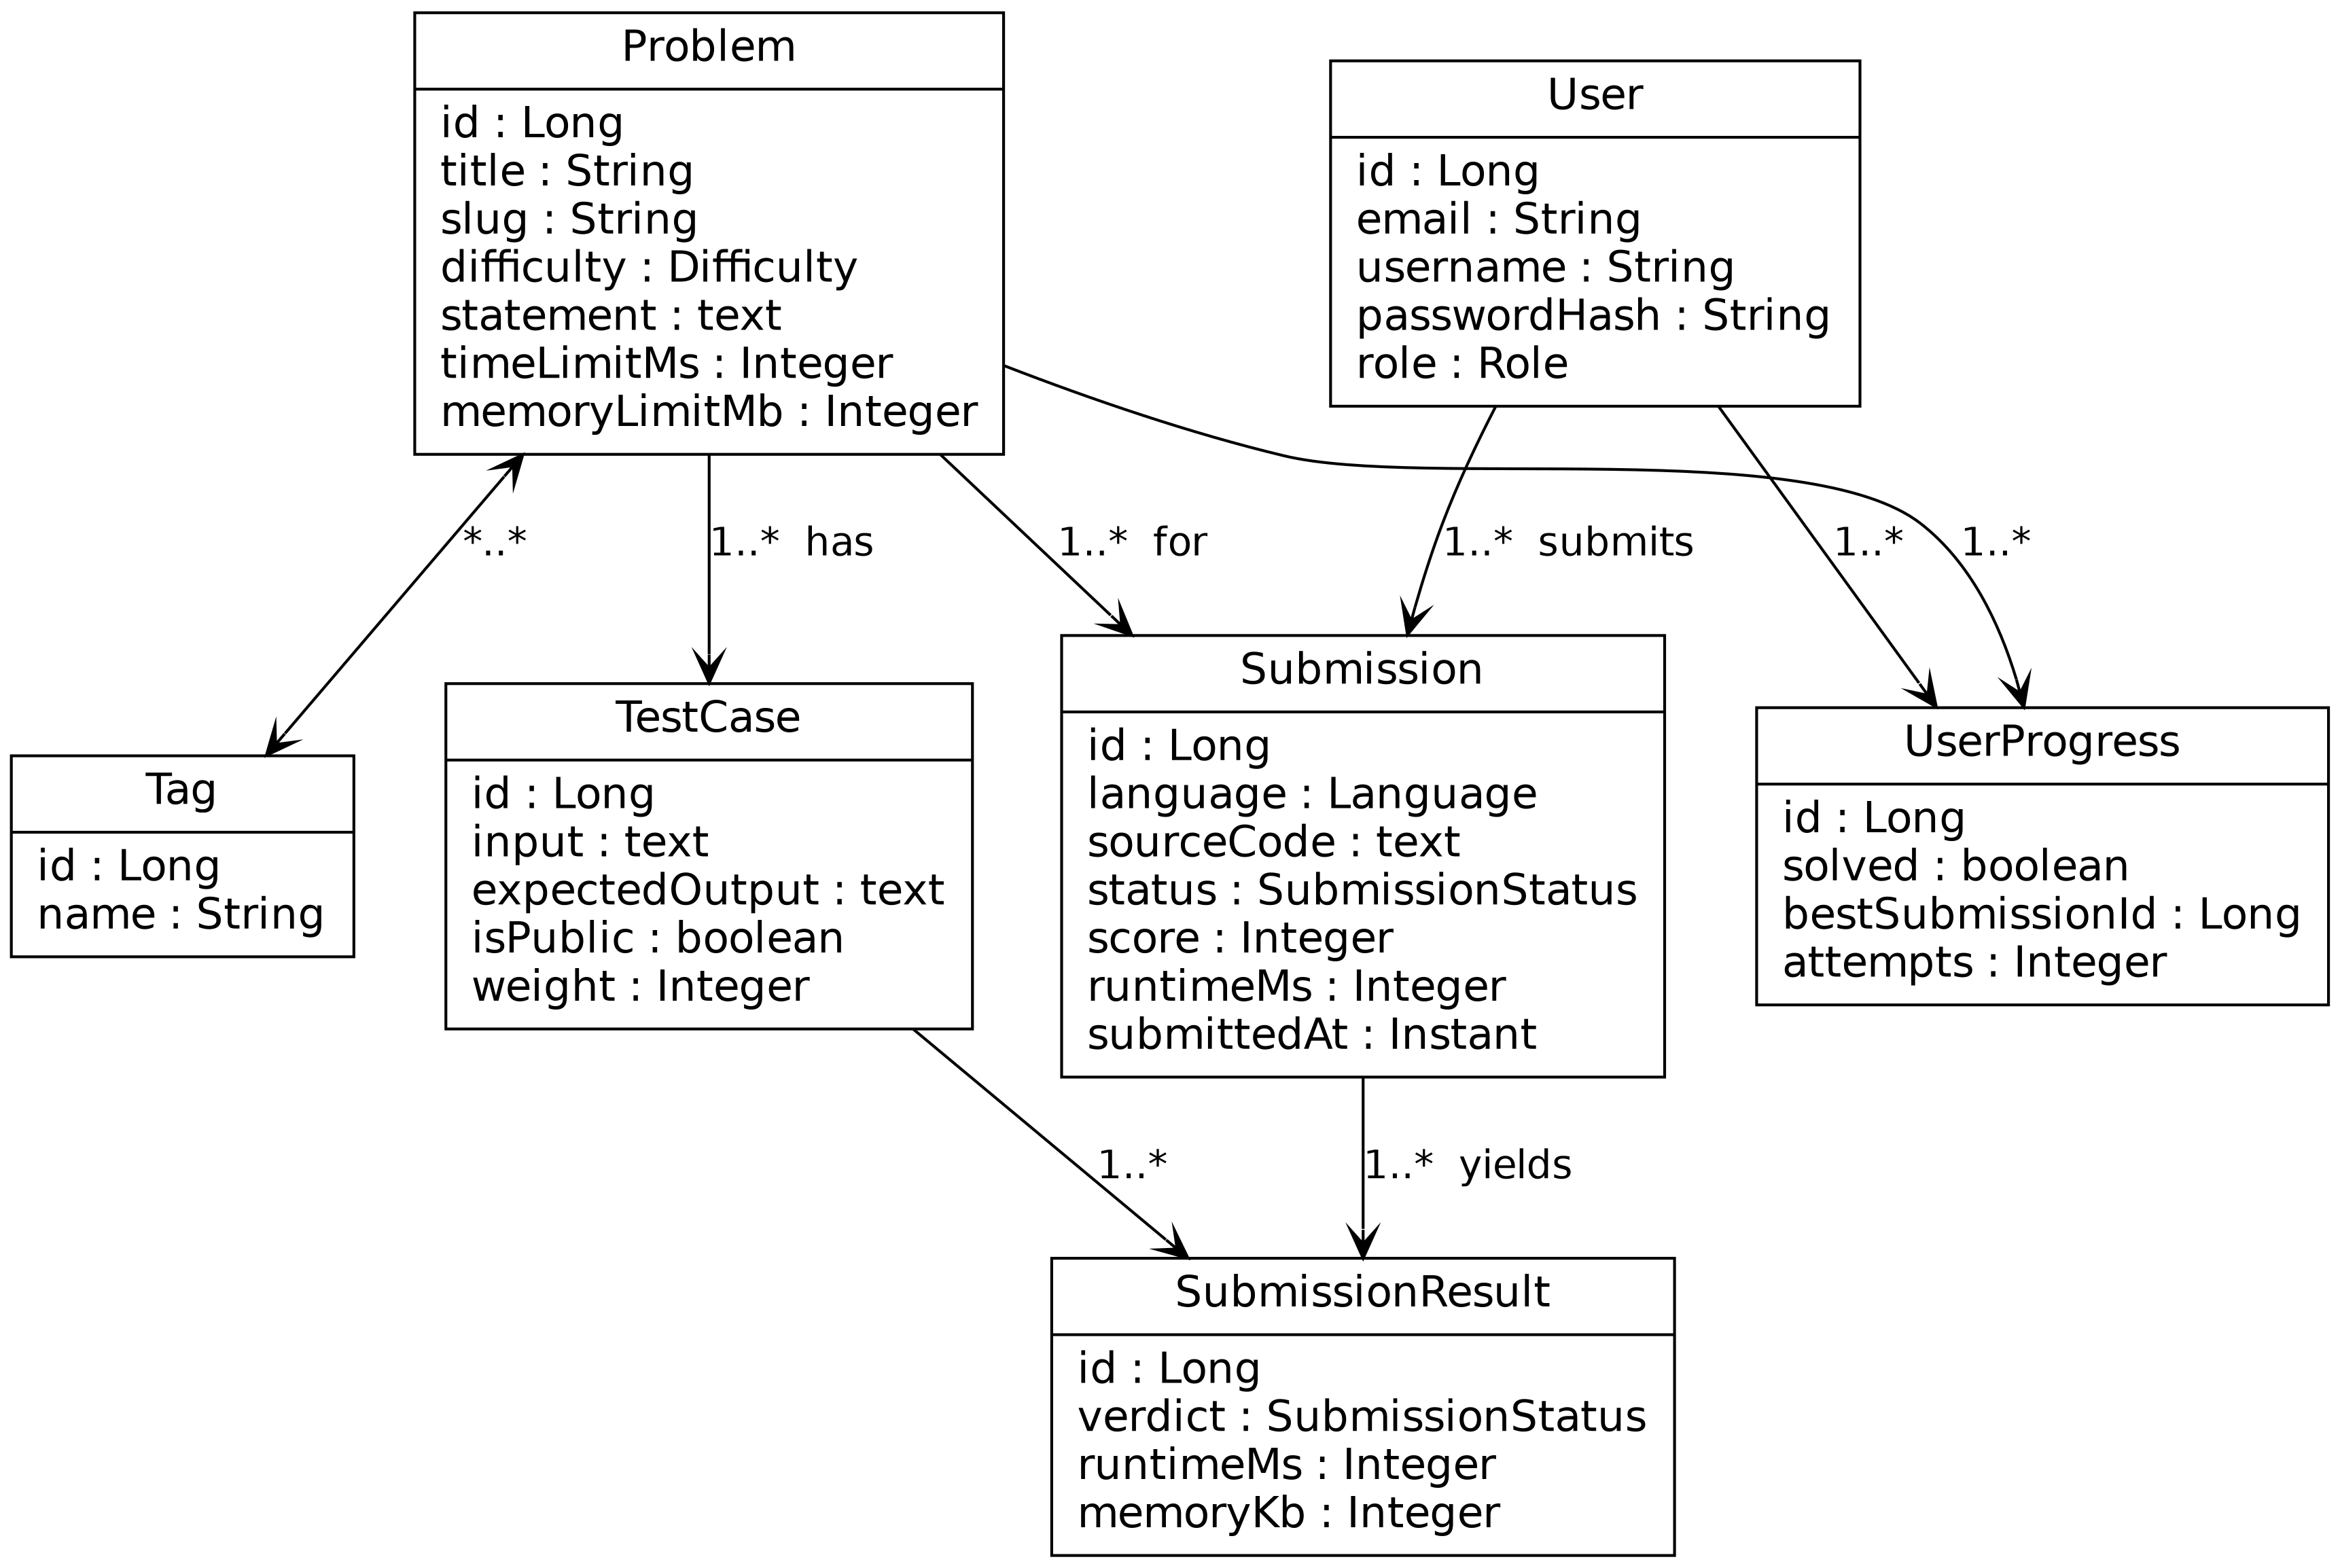
\includegraphics[width=0.92\textheight]{er_diagram.png}
  \caption{Entity relationship diagram of the persistence model, covering users and roles, problems, tags and test cases, and submissions, their per test results and user progress.}
  \label{fig:er}
\end{sidewaysfigure}

\section*{Authentication and Authorization}
Authentication was implemented as a stateless scheme based on JSON Web Tokens, so that the server need not keep any session state. When a user registers or logs in, the {\ttfamily AuthService} verifies the credentials, hashing and checking passwords with BCrypt, and the {\ttfamily JwtService} issues two signed tokens. The access token is short lived, expiring after fifteen minutes, and carries the user's identity and role; it is attached to every API request. The refresh token is long lived, expiring after seven days, and is used only to obtain a new access token when the current one expires. Both tokens are signed with an HMAC key read from an environment variable.

On each request, the {\ttfamily JwtAuthFilter} inspects the authorisation header, validates the token's signature and expiry and, if the token is valid, loads the user and places an authenticated principal into the security context for that request. Authorisation is then enforced declaratively in {\ttfamily SecurityConfig}, which permits public access to the authentication and read only problem endpoints while restricting problem creation, editing and deletion to administrators. A deliberate design point is that a missing or expired token results in an unauthorised response rather than a forbidden one, which allows the frontend to detect an expired token and refresh it automatically. The complete flow, including the automatic refresh that the frontend performs when it receives an unauthorised response, is shown in Figure~\ref{fig:jwt}.

\begin{sidewaysfigure}
  \centering
  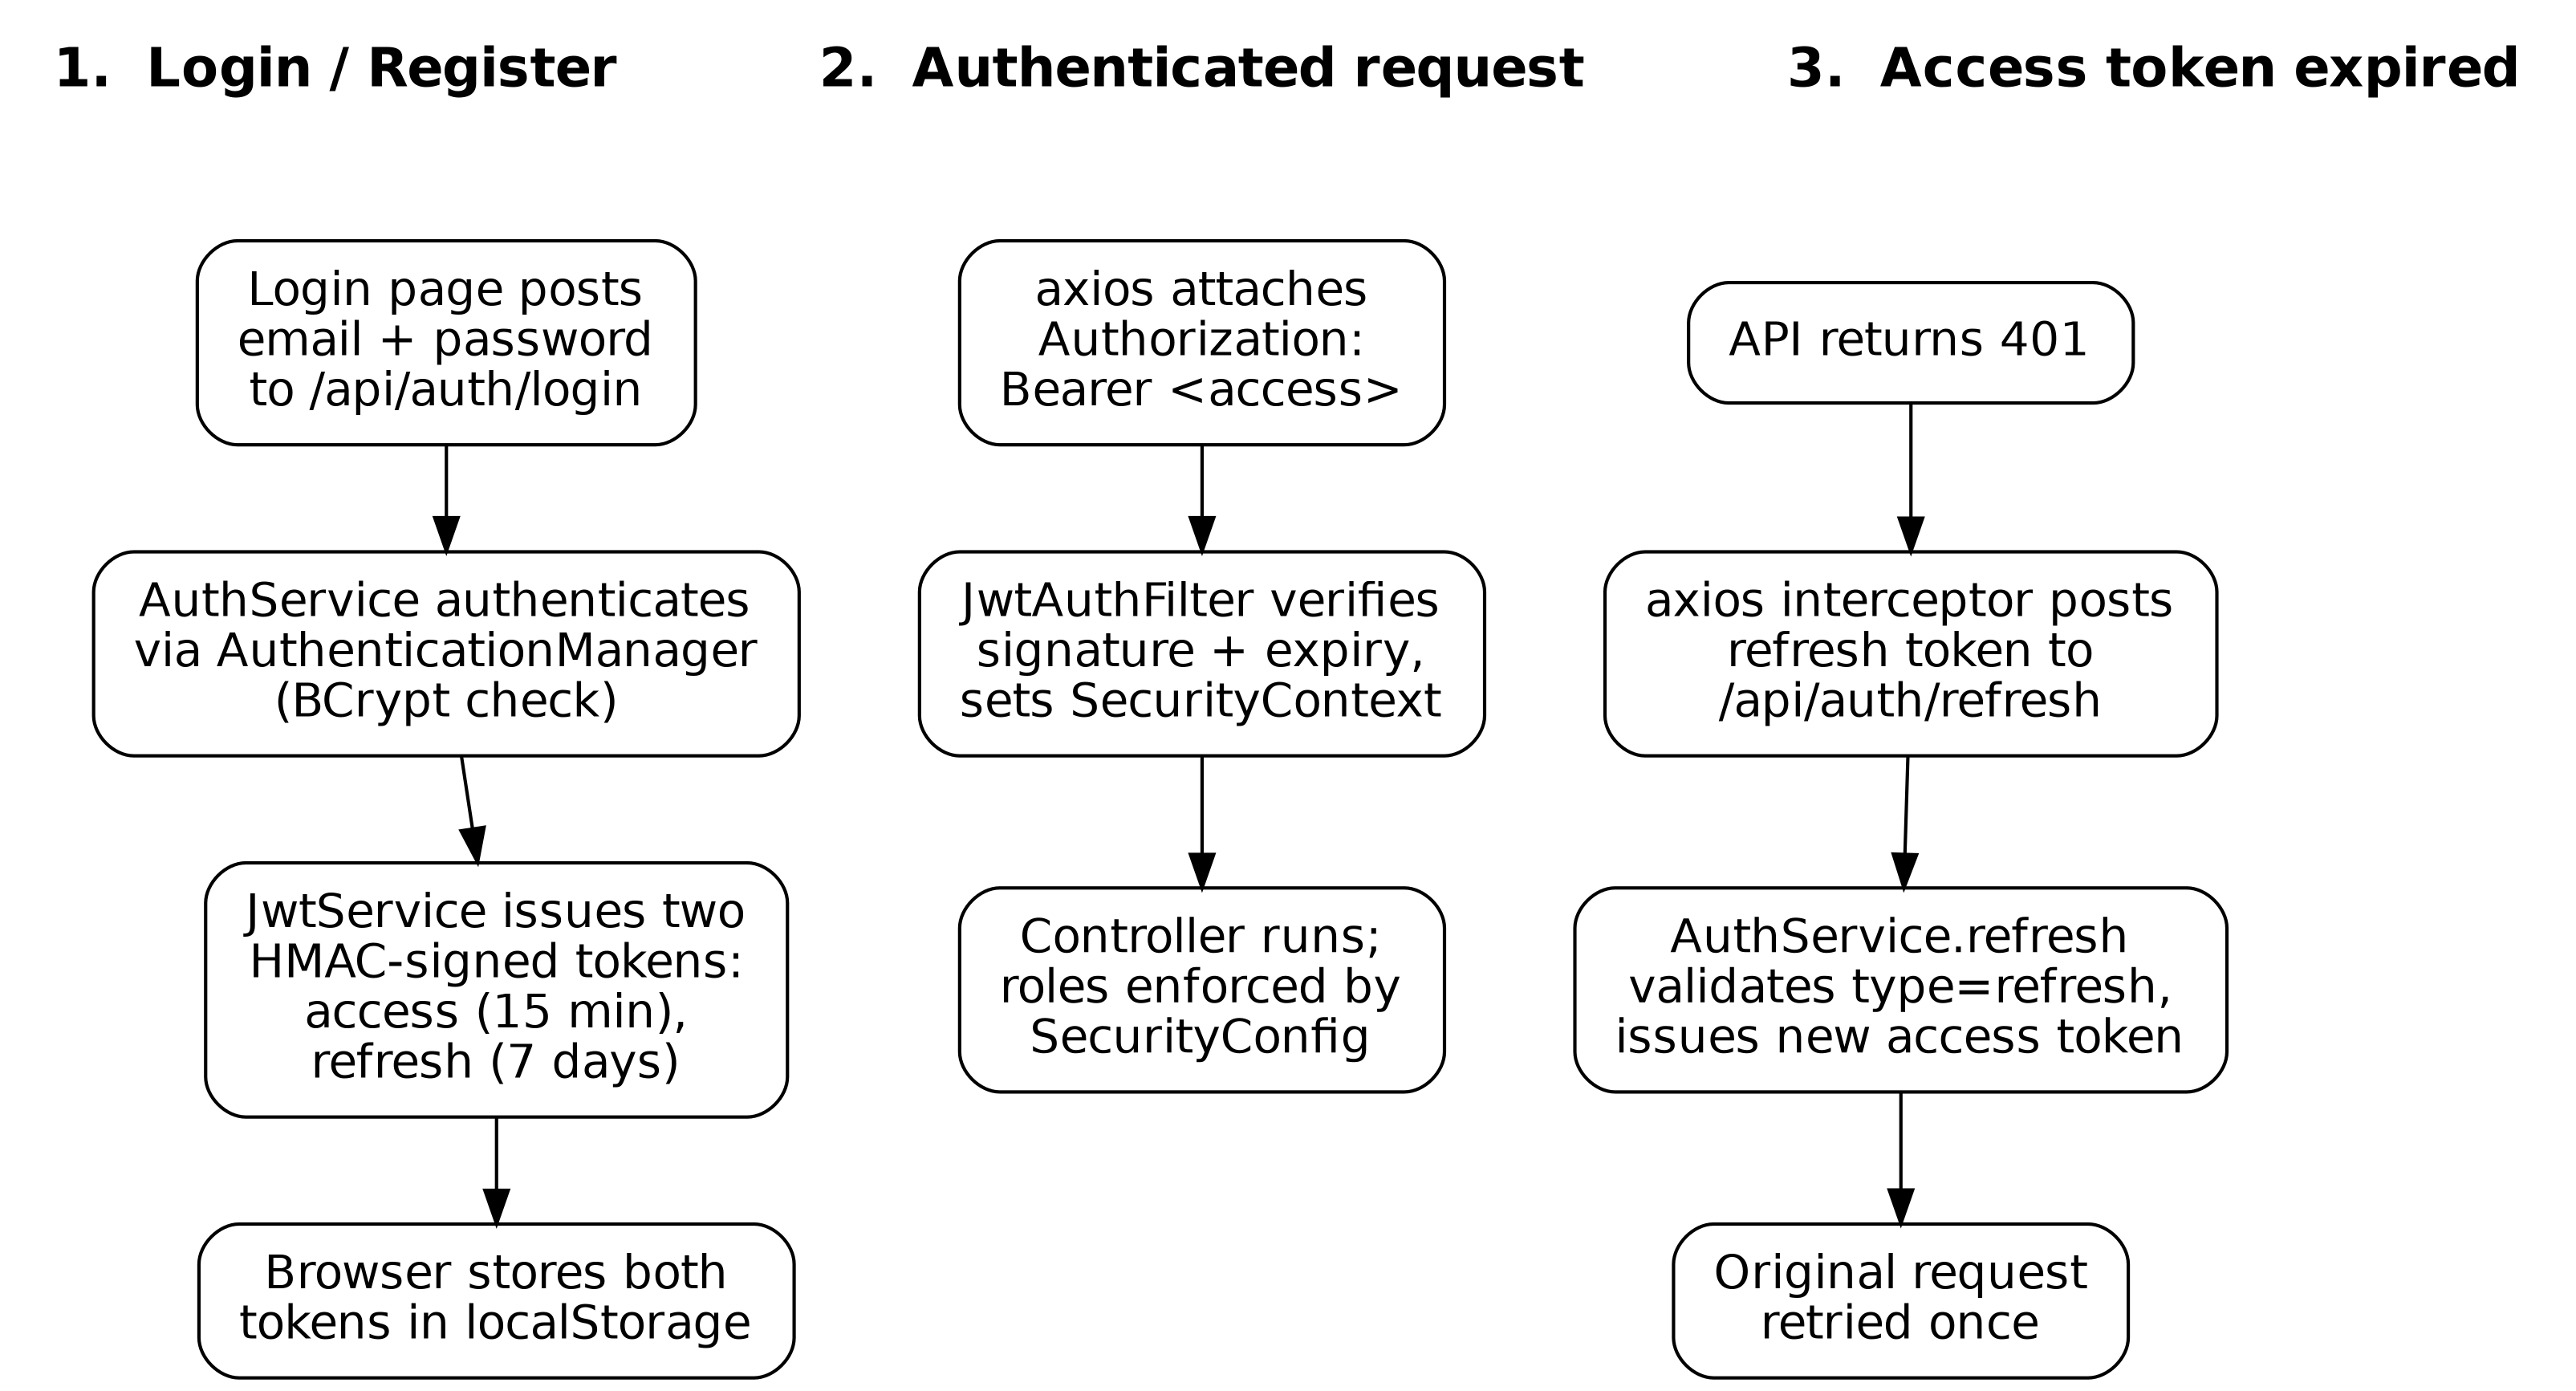
\includegraphics[width=0.92\textheight]{jwt_auth_flow.png}
  \caption{JSON Web Token flow, showing the issue of access and refresh tokens at login, their use on authenticated requests, and the automatic refresh when an access token has expired.}
  \label{fig:jwt}
\end{sidewaysfigure}

\section*{Problem Management APIs}
With authentication in place, the problem management APIs were implemented. These provide the usual create, read, update and delete operations, with all write operations restricted to administrators and the read operations open to everyone so that visitors can browse the problem set. Each problem has a difficulty of easy, medium or hard, a set of free form tags and a list of test cases, and the problem listing supports pagination so that large problem sets can be browsed a page at a time.

An important distinction in the design is between public and hidden test cases. Public test cases act as worked examples and are shown on the problem page so that users understand the expected input and output format, whereas hidden test cases are used only during judging and are never exposed through the public API. This is enforced at the service layer, where the endpoint that returns a problem to an ordinary user includes only the public test cases, while a separate administrator only endpoint returns the full set of test cases for editing. Problem titles are converted into unique slugs so that problems can be referenced by readable URLs, and editing a problem performs a full replacement of its test cases, which keeps the semantics of the administrator edit form simple and predictable.

\section*{Sandboxed Runner Images}
Because the platform executes untrusted code, each language is given its own minimal runner image rather than installing all the compilers into a single large image. Three images were built, one based on the GNU Compiler Collection for C++, one on an Eclipse Temurin Java Development Kit for Java and one on a slim Python image. Each image is deliberately small and contains only what is needed to compile and run programs in that language.

A key property shared by all three images is that they create and switch to an unprivileged user before running any submission. The sandbox user has a fixed non zero user identifier and no administrative rights, so that even if a submission were somehow able to interact with the container filesystem, it would not do so as the root user. Keeping the images minimal also reduces the attack surface, since there are fewer tools available inside the container for a malicious program to misuse. These images are referenced by name from the backend, which launches them with a strict set of isolation flags described in the next section.

\section*{Judge Engine}
The judge engine is the core of the platform and was the largest single activity of the internship. When a submission is received it is saved with a pending status and judging is triggered in the background. The judge first creates a private workspace directory for the submission and writes the source code into it. For the compiled languages a separate compile step is run, and if compilation fails the submission is marked as a compile error and the compiler output is stored so that it can be shown to the user. Python, although interpreted, is passed through a byte compilation step so that a syntax error is reported as a compile error in the same way as for the other languages. If compilation succeeds, the judge runs the program once for each test case, feeding the test input on standard input and capturing the output. The overall sequence, from the user pressing submit to the verdict appearing on the submission page, is shown in Figure~\ref{fig:lifecycle}.

\begin{figure}[htbp]
  \centering
  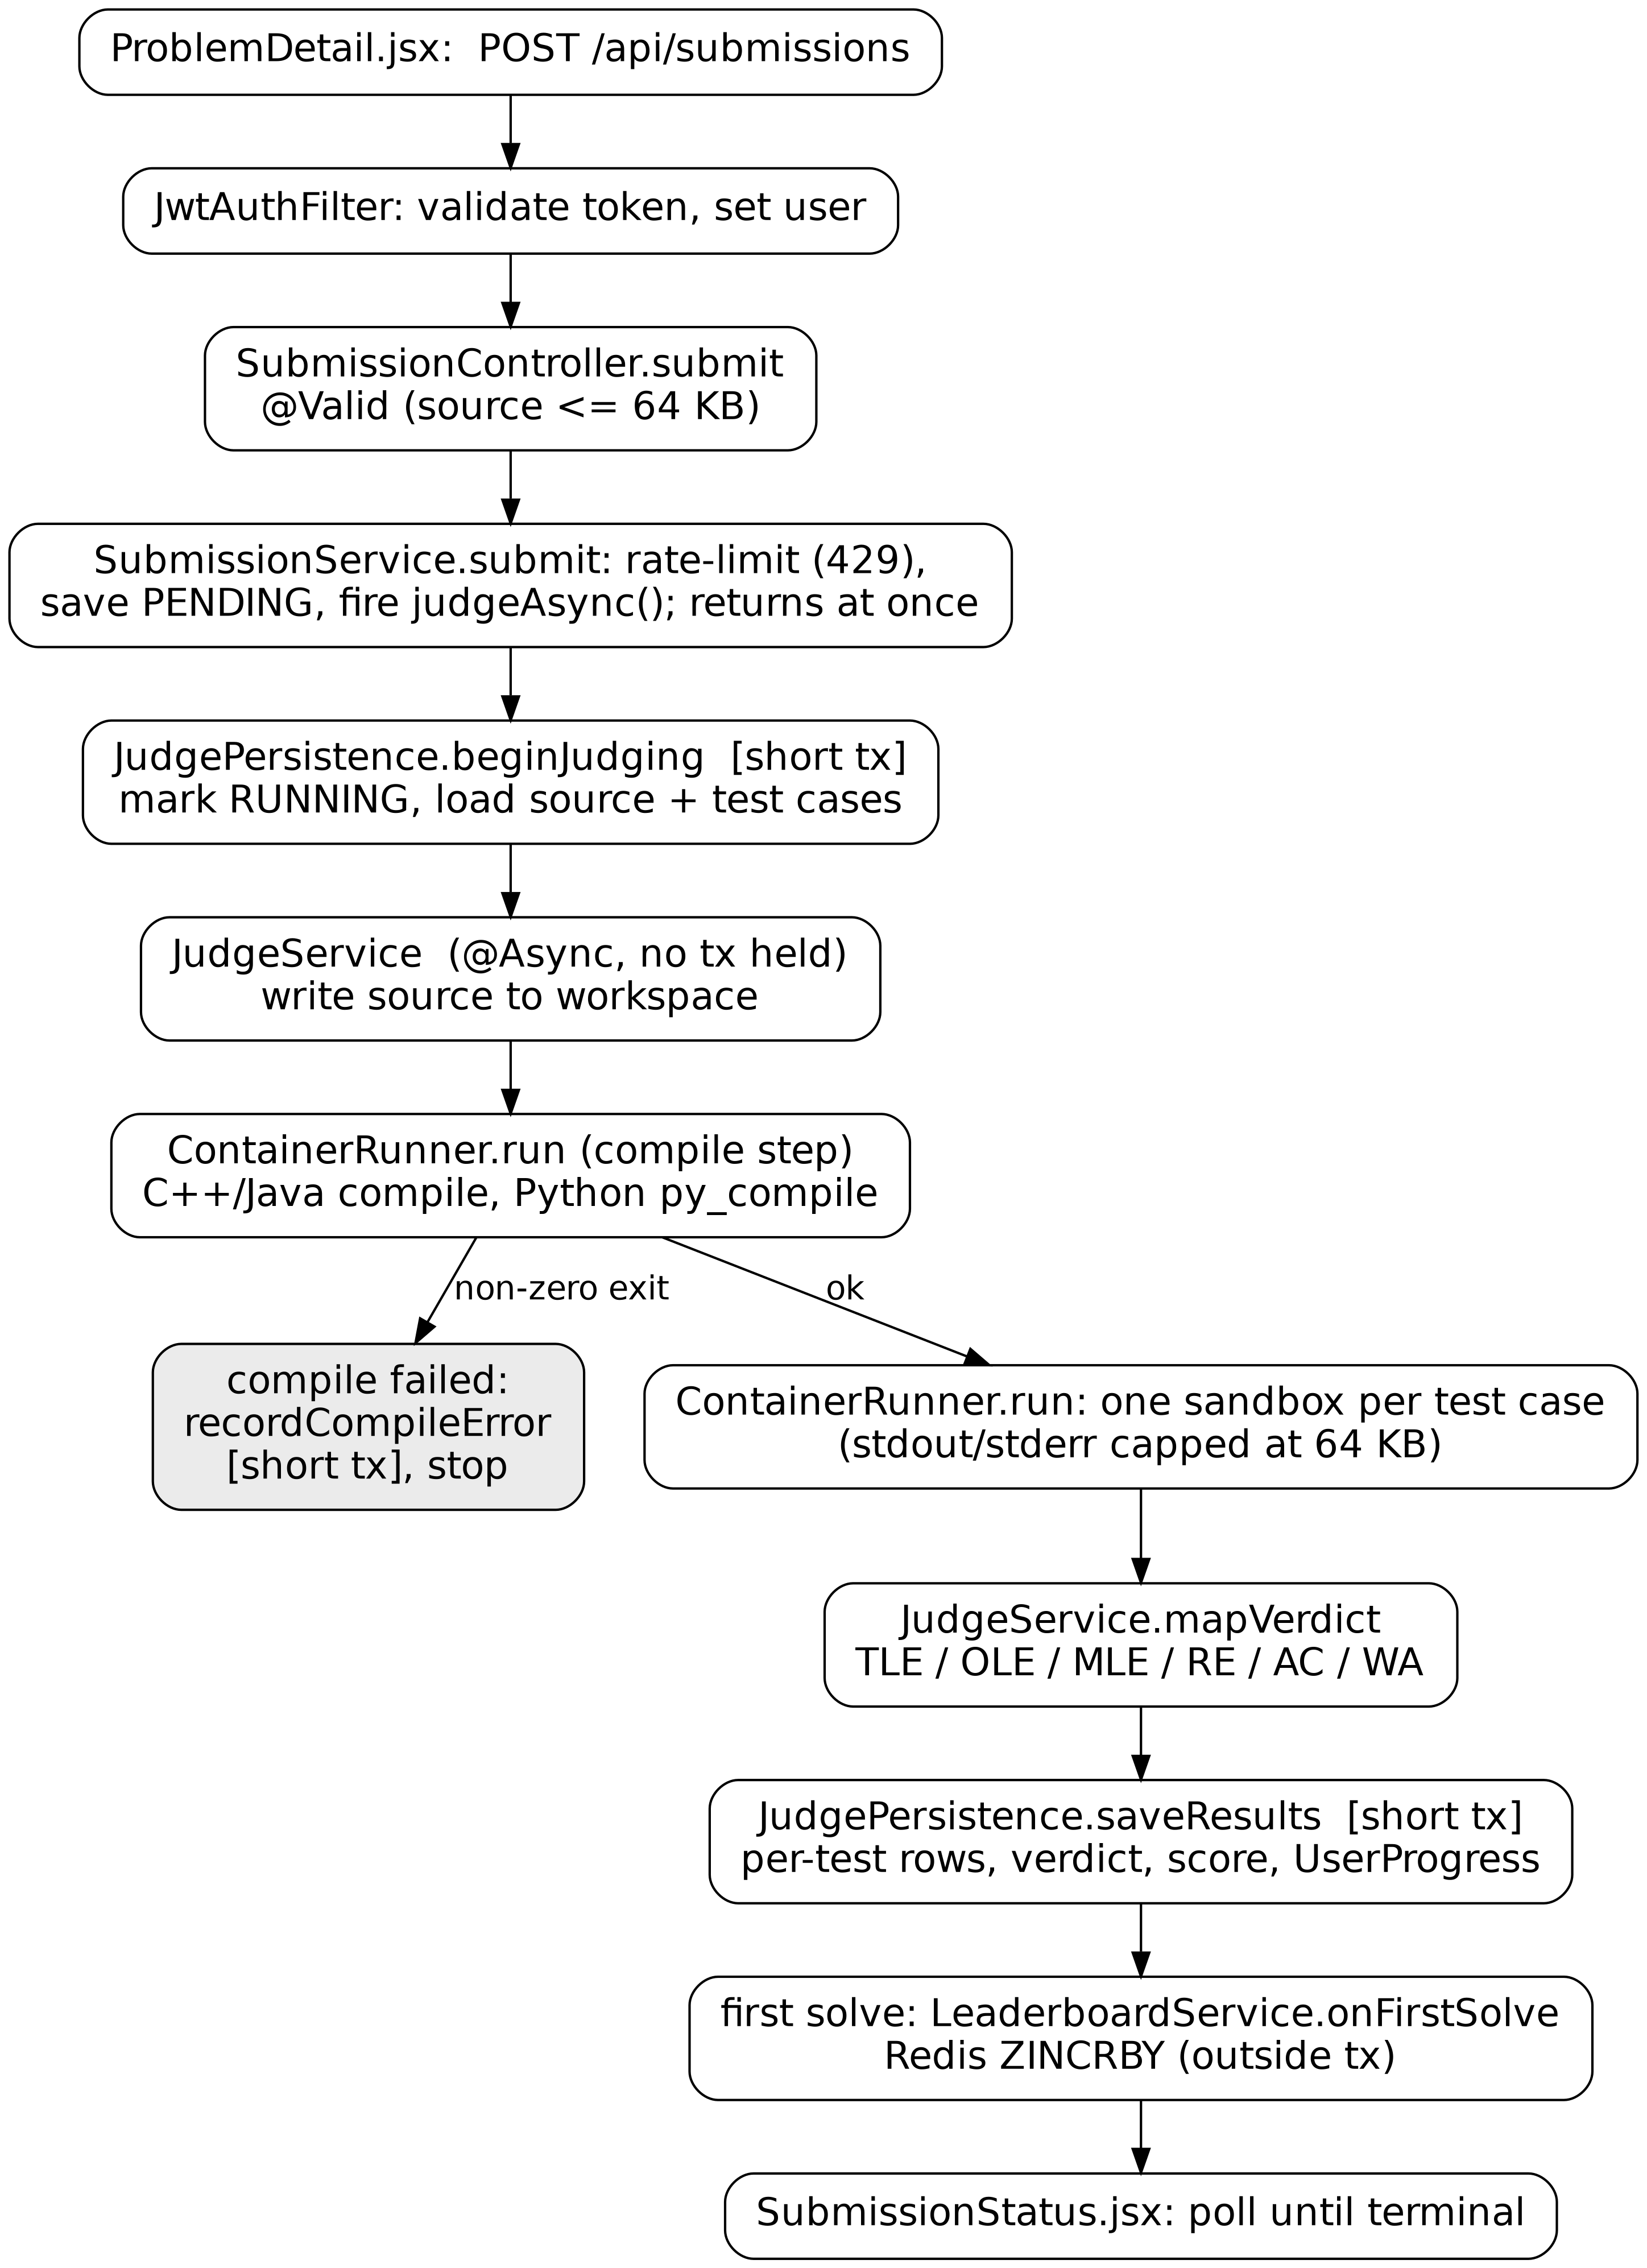
\includegraphics[width=\textwidth]{judge_lifecycle.png}
  \caption{Lifecycle of a submission, naming the main classes and methods involved from the submit request through compilation and per test execution to the stored verdict and the polling submission page.}
  \label{fig:lifecycle}
\end{figure}

Every compile step and every test case is executed in a fresh Docker container that is launched with a strict set of isolation and resource control flags, shown in Listing~\ref{lst:dockerrun}. These flags are what make it safe to run untrusted code, and each one guards against a specific category of misbehaviour, as summarised in Table~\ref{tab:flags}.

\begin{lstlisting}[caption={The argument list used to launch each sandbox container.},label={lst:dockerrun}]
docker run --rm --name judge-<uuid> -i \
  --network=none \
  --memory=256m --memory-swap=256m \
  --cpus=1 --pids-limit=64 \
  --read-only --tmpfs /tmp:rw,size=32m \
  -v <workdir>:/box:rw -w /box \
  <runner-image> <compile-or-run-command>
\end{lstlisting}

\begin{table}[htbp]
  \centering
  \caption{The main sandbox flags and the misbehaviour each one prevents.}
  \label{tab:flags}
  \begin{tabular}{|p{0.42\textwidth}|p{0.5\textwidth}|}
    \hline
    \textbf{Flag} & \textbf{What it protects against} \\
    \hline
    {\ttfamily --network=none} & Removes all network access, preventing data exfiltration and any outbound connections. \\
    \hline
    {\ttfamily --memory} / {\ttfamily --memory-swap} & Caps memory with no swap; exceeding it causes an out of memory kill, reported as memory limit exceeded. \\
    \hline
    {\ttfamily --cpus=1} & Limits CPU so that one submission cannot starve others of processing time. \\
    \hline
    {\ttfamily --pids-limit=64} & Caps the number of processes, defeating fork bombs. \\
    \hline
    {\ttfamily --read-only} with {\ttfamily --tmpfs /tmp} & Makes the root filesystem read only with only a small scratch area writable, preventing tampering and large disk writes. \\
    \hline
    non root sandbox user & Runs the code unprivileged, so it never executes as root inside the container. \\
    \hline
    {\ttfamily -v <workdir>:/box} & Shares only the submission's own workspace, so code cannot see other submissions or host files. \\
    \hline
    unique {\ttfamily --name} with forced removal & Allows a timed out or runaway container to be killed and removed, leaving no orphaned containers. \\
    \hline
  \end{tabular}
\end{table}

Once a program has run, its outcome is translated into a verdict. A wall clock timeout results in time limit exceeded, an out of memory kill in memory limit exceeded, and a program that writes more output than a fixed cap in output limit exceeded. Any other non zero exit is treated as a runtime error, while a clean exit leads to a comparison of the program output against the expected output, giving either accepted or wrong answer. The output comparison is lenient about insignificant whitespace, normalising line endings and trailing spaces so that a correct answer is not rejected for a trailing newline, while still treating differences within a line as significant. To ensure that a program which prints endlessly cannot exhaust the judge's memory, the captured output is bounded at sixty four kilobytes and is drained on dedicated threads, which also avoids a deadlock that would otherwise occur when a program fills the output buffer faster than it is read.

Reliability of the judging process received particular attention. On a timeout or an output flood the container is not merely abandoned; it is explicitly killed and removed by name so that no orphaned containers are left running and consuming resources, and the per submission workspace is deleted once judging finishes. A subtle but important design decision concerns database transactions. In an early version the entire judging routine was both asynchronous and transactional, which meant that a single database transaction, and the database connection backing it, was held open for the whole duration of judging, across every slow container invocation. This does not scale, because under load the connection pool would quickly be exhausted. The judging was therefore restructured so that the asynchronous method holds no transaction at all, and all database work is performed through a separate component whose methods each open a short transaction: one to mark the submission as running and read the inputs, and one to save the final verdict and the per test results. Keeping this logic in a separate component was necessary rather than cosmetic, because Spring applies the transactional behaviour through a proxy, and a call from one method of a class to another method of the same class would bypass that proxy and silently ignore the transaction. Finally, if judging fails unexpectedly for any reason, the submission is moved to an internal error state rather than being left stuck as running.

\section*{Asynchronous Submission Processing and Rate Limiting}
Judging a submission can take several seconds, far too long for the user to wait on a single HTTP request. The submission endpoint therefore saves the submission, starts judging asynchronously using the Spring {\ttfamily @Async} mechanism and returns immediately, after which the frontend polls for the result. This keeps the API responsive and allows several submissions to be judged concurrently. Because judging runs on a background thread, care was taken to ensure that all the information it needs is read from the database up front and that its outcome is written back through short transactions, as described above.

To prevent abuse and to protect the judge from being overwhelmed by a single user, a per user submission rate limit was added. If a user attempts to submit again within a short window of the previous submission, the request is rejected with a too many requests response and a clear message indicating how long to wait, which the frontend displays. The limit is currently held in memory, which is appropriate for a single instance deployment; in a multi instance deployment it would be moved into Redis so that the window is shared across all instances. This rate limiting, together with the maximum source code size enforced by request validation, keeps the submission path well behaved.

\section*{Leaderboard}
The leaderboard ranks users by the number of distinct problems they have solved. Although PostgreSQL remains the source of truth for all data, computing the ranking by scanning the database on every request would not scale, so the leaderboard is served from a Redis sorted set in which the members are user identifiers and the scores are solved counts. Reading the top of the leaderboard is then a single sorted set range query, and the usernames for the returned identifiers are resolved in one batch query rather than one lookup per row.

The sorted set is kept in step with the database in two ways. When a user solves a problem for the very first time, and only then, their score is incremented; a repeated correct submission for a problem that has already been solved does not change the score. This is driven by the user progress record, which distinguishes a first solve from a resubmission. To guard against the sorted set drifting out of step, for example after a restart, it is rebuilt from the database when the application starts, so that Redis always begins as an accurate cache of the authoritative data in PostgreSQL. The design also degrades gracefully: if Redis is unavailable, the leaderboard falls back to computing the ranking directly from PostgreSQL and logs a warning, with the Redis timeouts kept short so that the fallback is fast rather than leaving the request hanging.

\section*{Frontend Development}
The frontend was built as a React single page application using Vite as the build tool, with React Router for navigation and an Axios based API client. Authentication state is held in a context that stores the tokens and the current user and attaches the access token to every request; the same client transparently refreshes an expired access token and retries the original request. The login and registration pages are shown in Figure~\ref{fig:login} and Figure~\ref{fig:register}.

\begin{figure}[htbp]
  \centering
  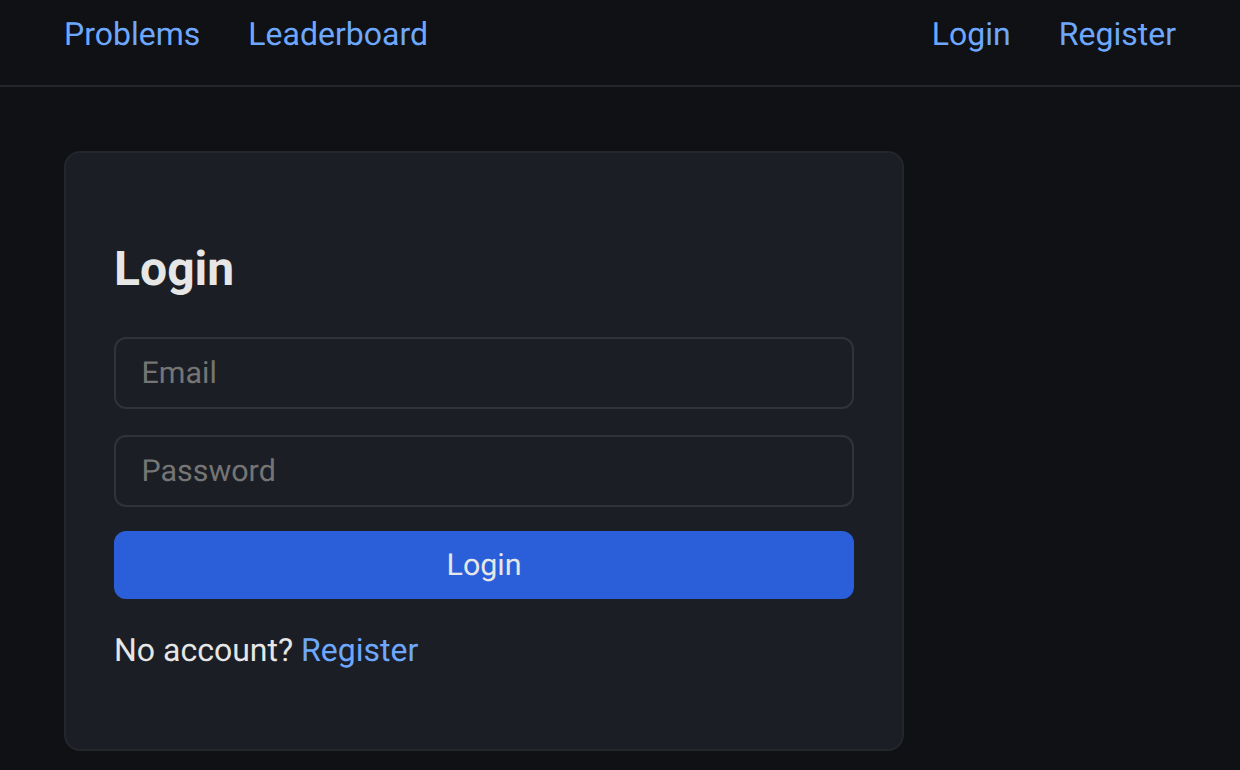
\includegraphics[width=\textwidth]{ui_login.png}
  \caption{The login page.}
  \label{fig:login}
\end{figure}

\begin{figure}[htbp]
  \centering
  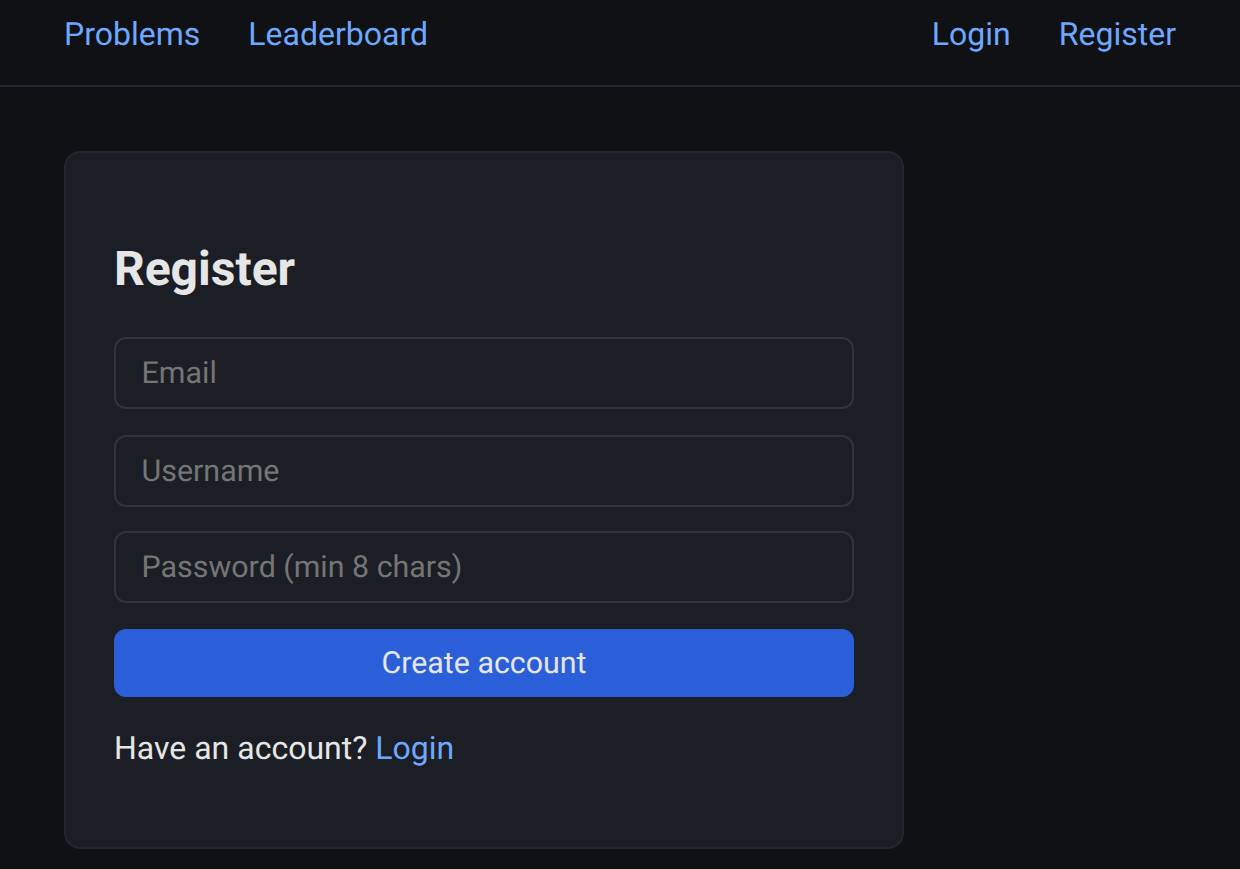
\includegraphics[width=\textwidth]{ui_register.png}
  \caption{The registration page.}
  \label{fig:register}
\end{figure}

The problem list presents the available problems with their difficulty and tags, and selecting a problem opens the problem detail page, which shows the statement, the public sample tests and a Monaco based code editor with language specific templates for C++, Java and Python. Figure~\ref{fig:list} and Figure~\ref{fig:detail} show these two pages.

\begin{figure}[htbp]
  \centering
  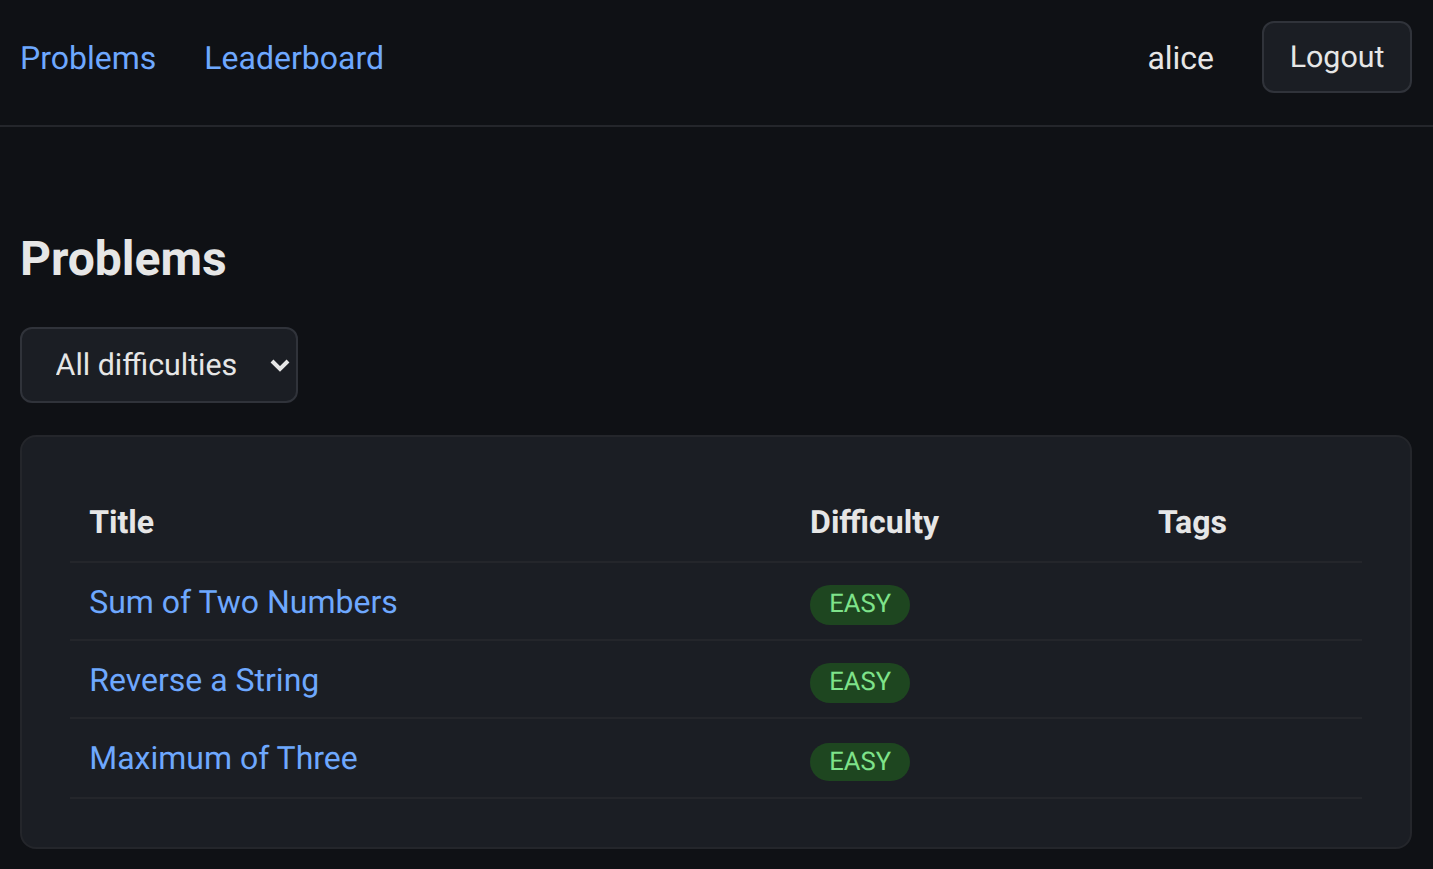
\includegraphics[width=\textwidth]{ui_problem_list.png}
  \caption{The problem list, showing difficulty and tags for each problem.}
  \label{fig:list}
\end{figure}

\begin{figure}[htbp]
  \centering
  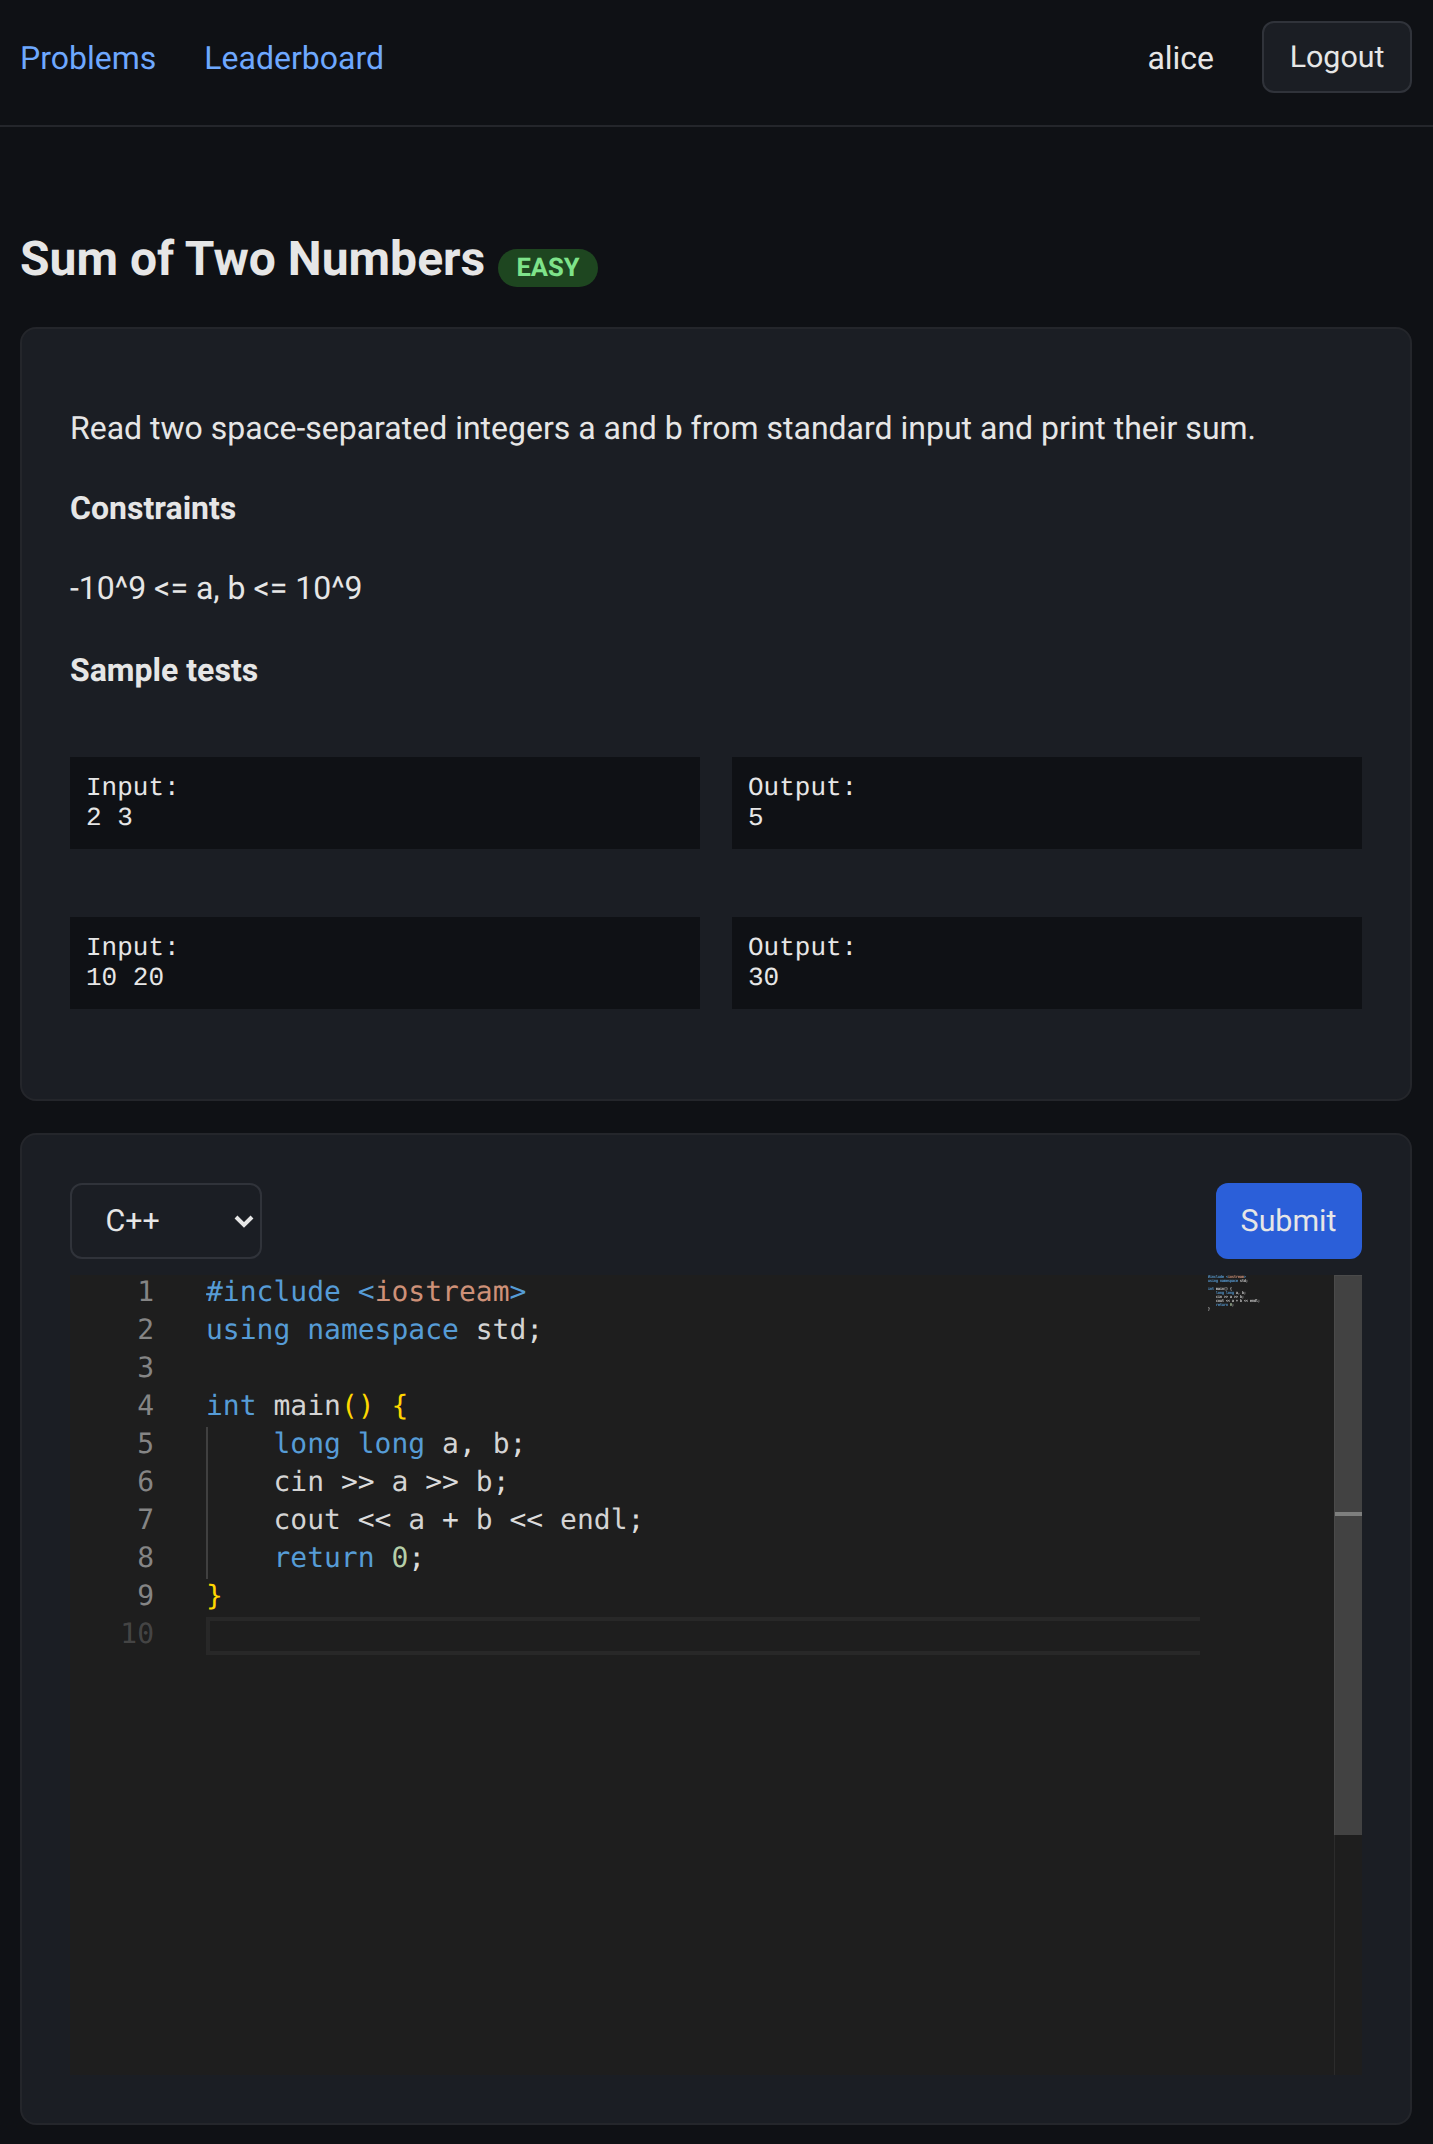
\includegraphics[width=0.85\textwidth]{ui_problem_detail.png}
  \caption{The problem detail page, with the statement, sample tests and the Monaco code editor holding a candidate solution.}
  \label{fig:detail}
\end{figure}

After a solution is submitted, the user is taken to the submission status page, which polls the backend every one and a half seconds until a final verdict is reached and then displays the overall verdict together with a per test breakdown. Figure~\ref{fig:accepted} shows the page for an accepted submission, Figure~\ref{fig:ce} shows one that failed to compile (with the compiler output shown directly so the user can see what went wrong), and Figure~\ref{fig:tle} shows one that exceeded the time limit.

\begin{figure}[htbp]
  \centering
  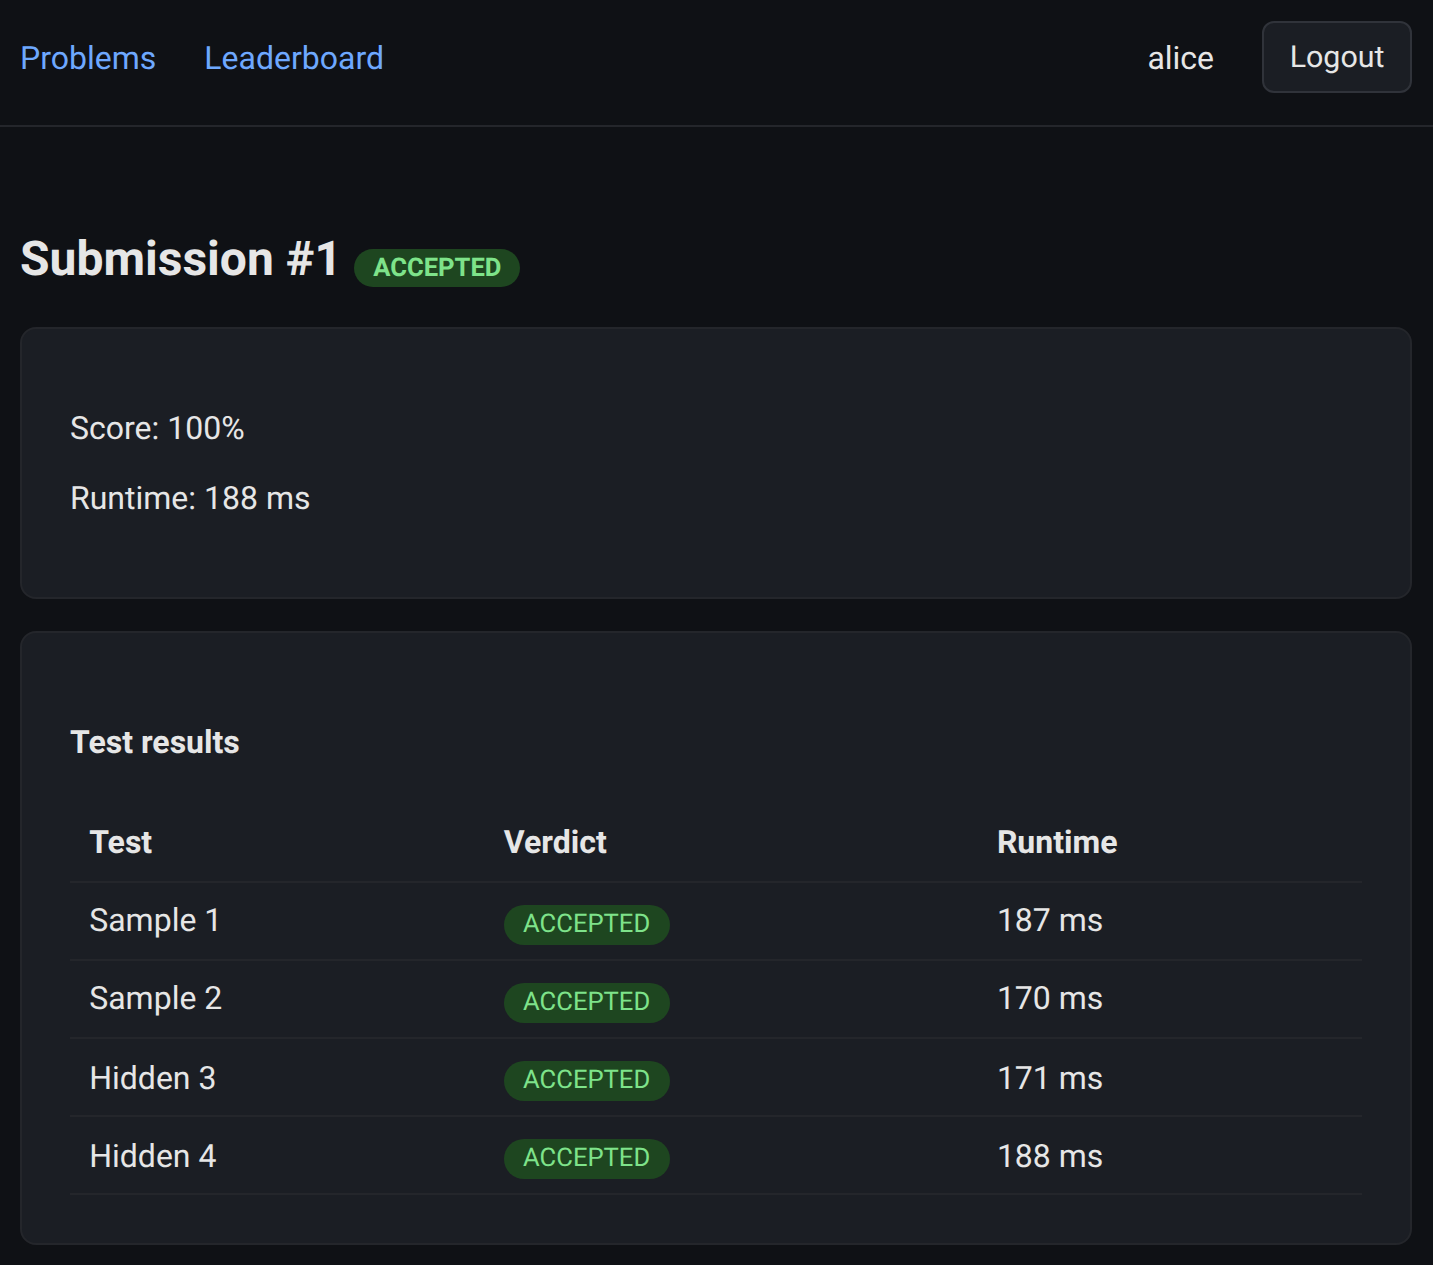
\includegraphics[width=\textwidth]{ui_submission_accepted.png}
  \caption{An accepted submission, showing the score, runtime and the per test result table.}
  \label{fig:accepted}
\end{figure}

\begin{figure}[htbp]
  \centering
  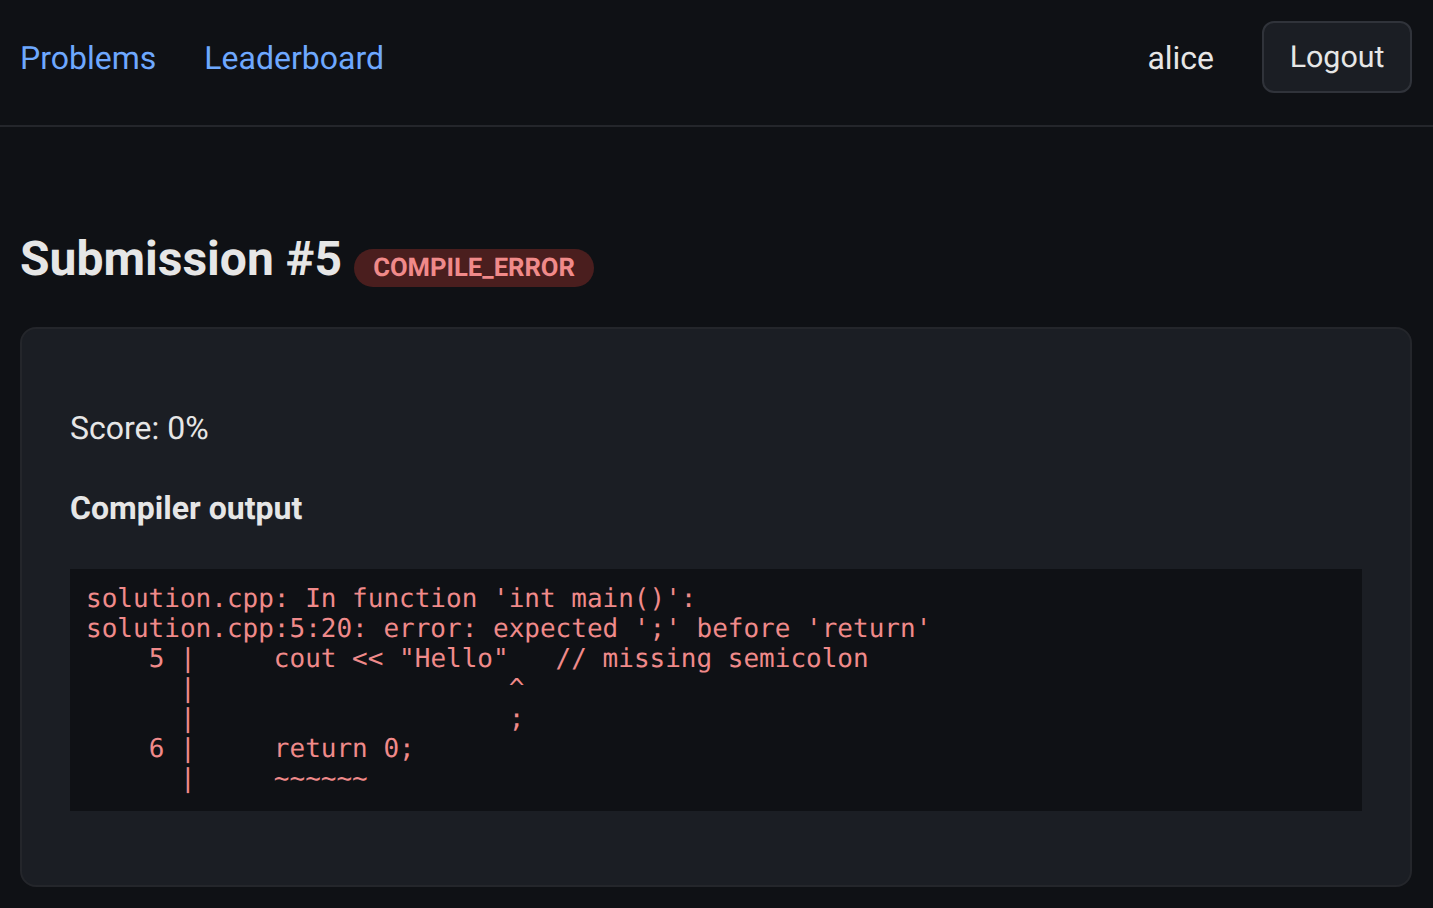
\includegraphics[width=\textwidth]{ui_submission_compile_error.png}
  \caption{A submission that failed to compile, with the stored compiler output shown to the user.}
  \label{fig:ce}
\end{figure}

\begin{figure}[htbp]
  \centering
  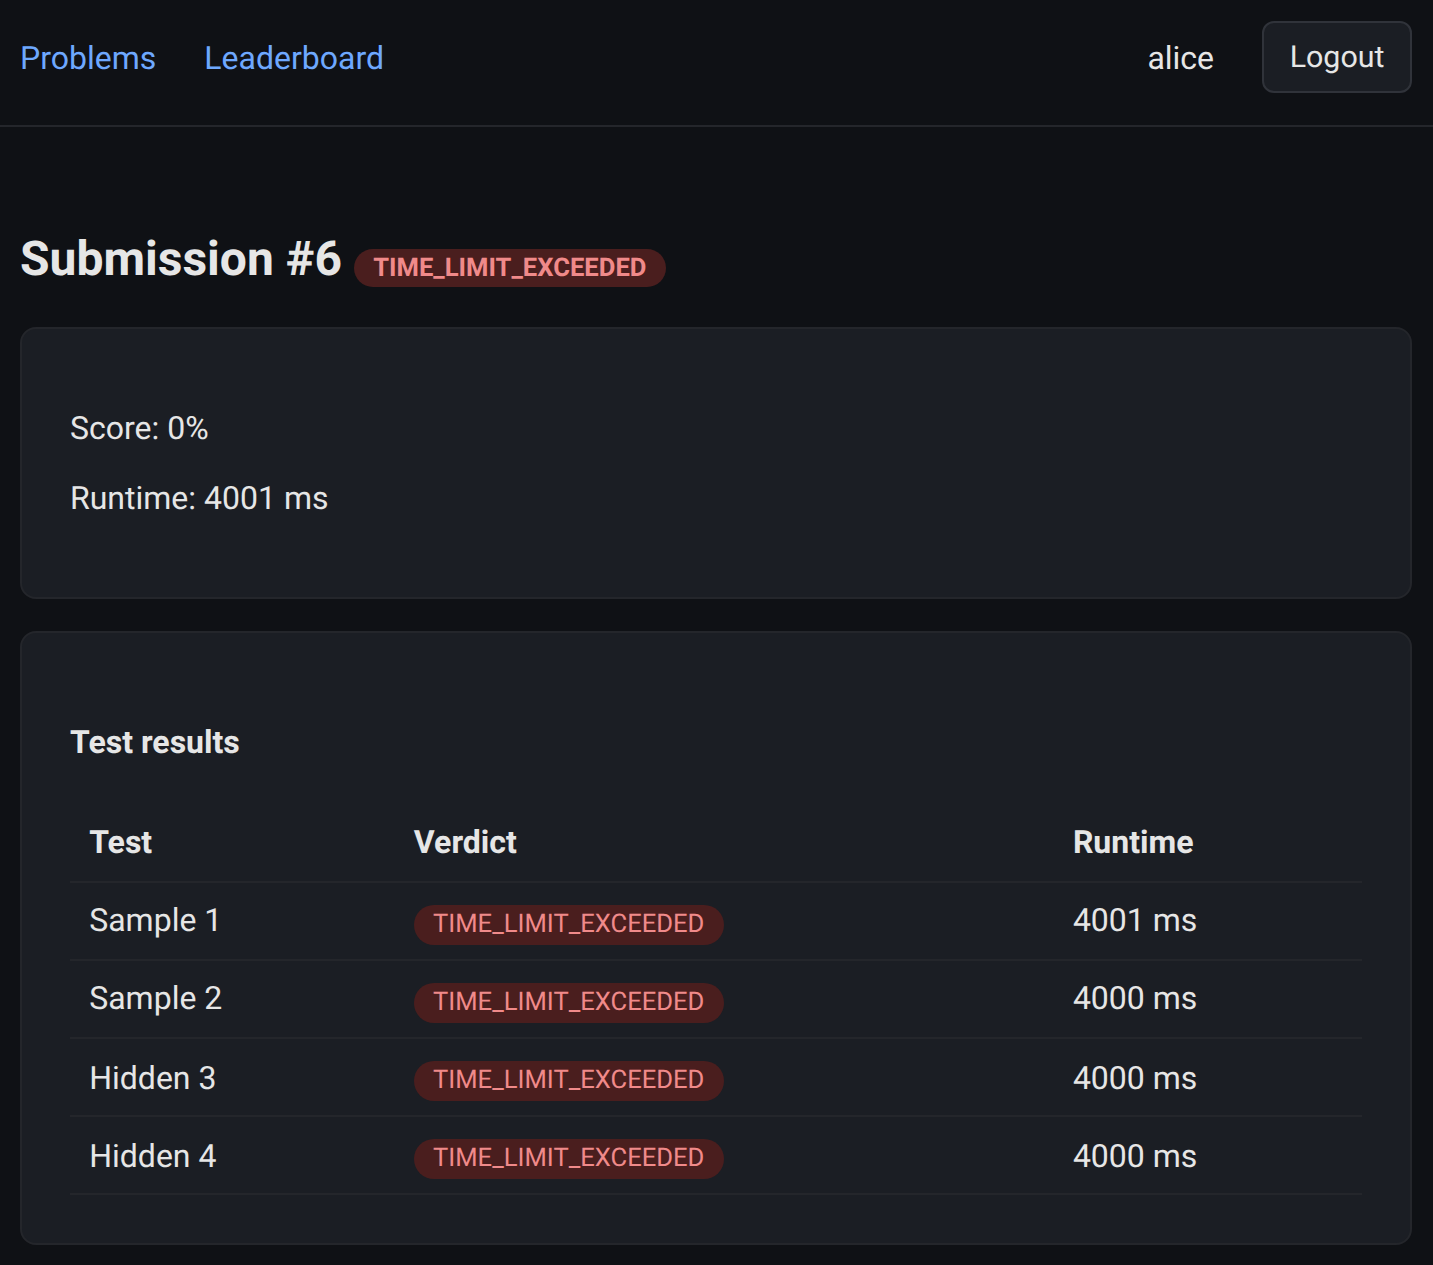
\includegraphics[width=\textwidth]{ui_submission_tle.png}
  \caption{A submission that exceeded the time limit.}
  \label{fig:tle}
\end{figure}

The leaderboard page, shown in Figure~\ref{fig:leaderboard}, lists the top users by number of problems solved, and the administrator pages, shown in Figure~\ref{fig:adminnew} and Figure~\ref{fig:adminedit}, allow problems to be created and edited, including their test cases and the public or hidden flag for each one.

\begin{figure}[htbp]
  \centering
  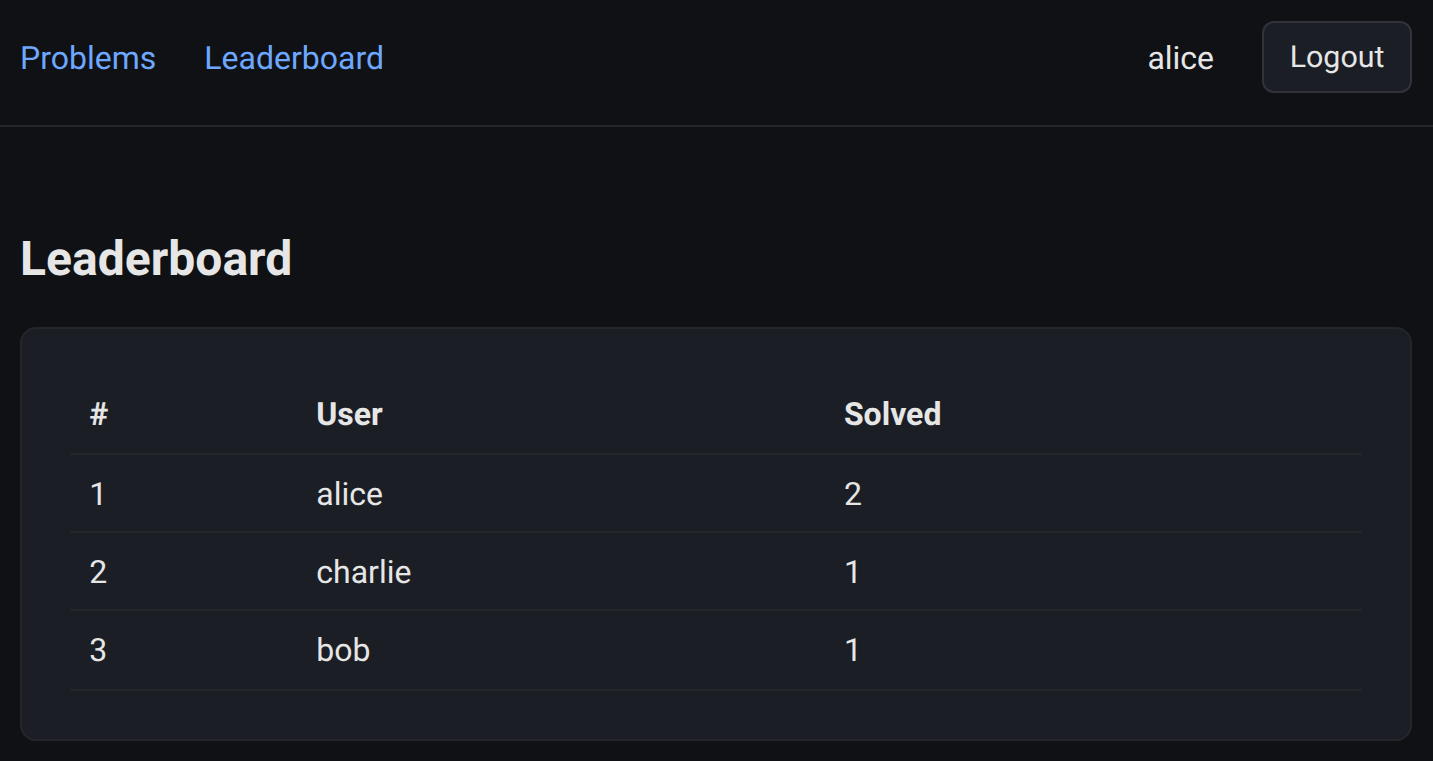
\includegraphics[width=\textwidth]{ui_leaderboard.png}
  \caption{The leaderboard, ranking users by the number of problems solved.}
  \label{fig:leaderboard}
\end{figure}

\begin{figure}[htbp]
  \centering
  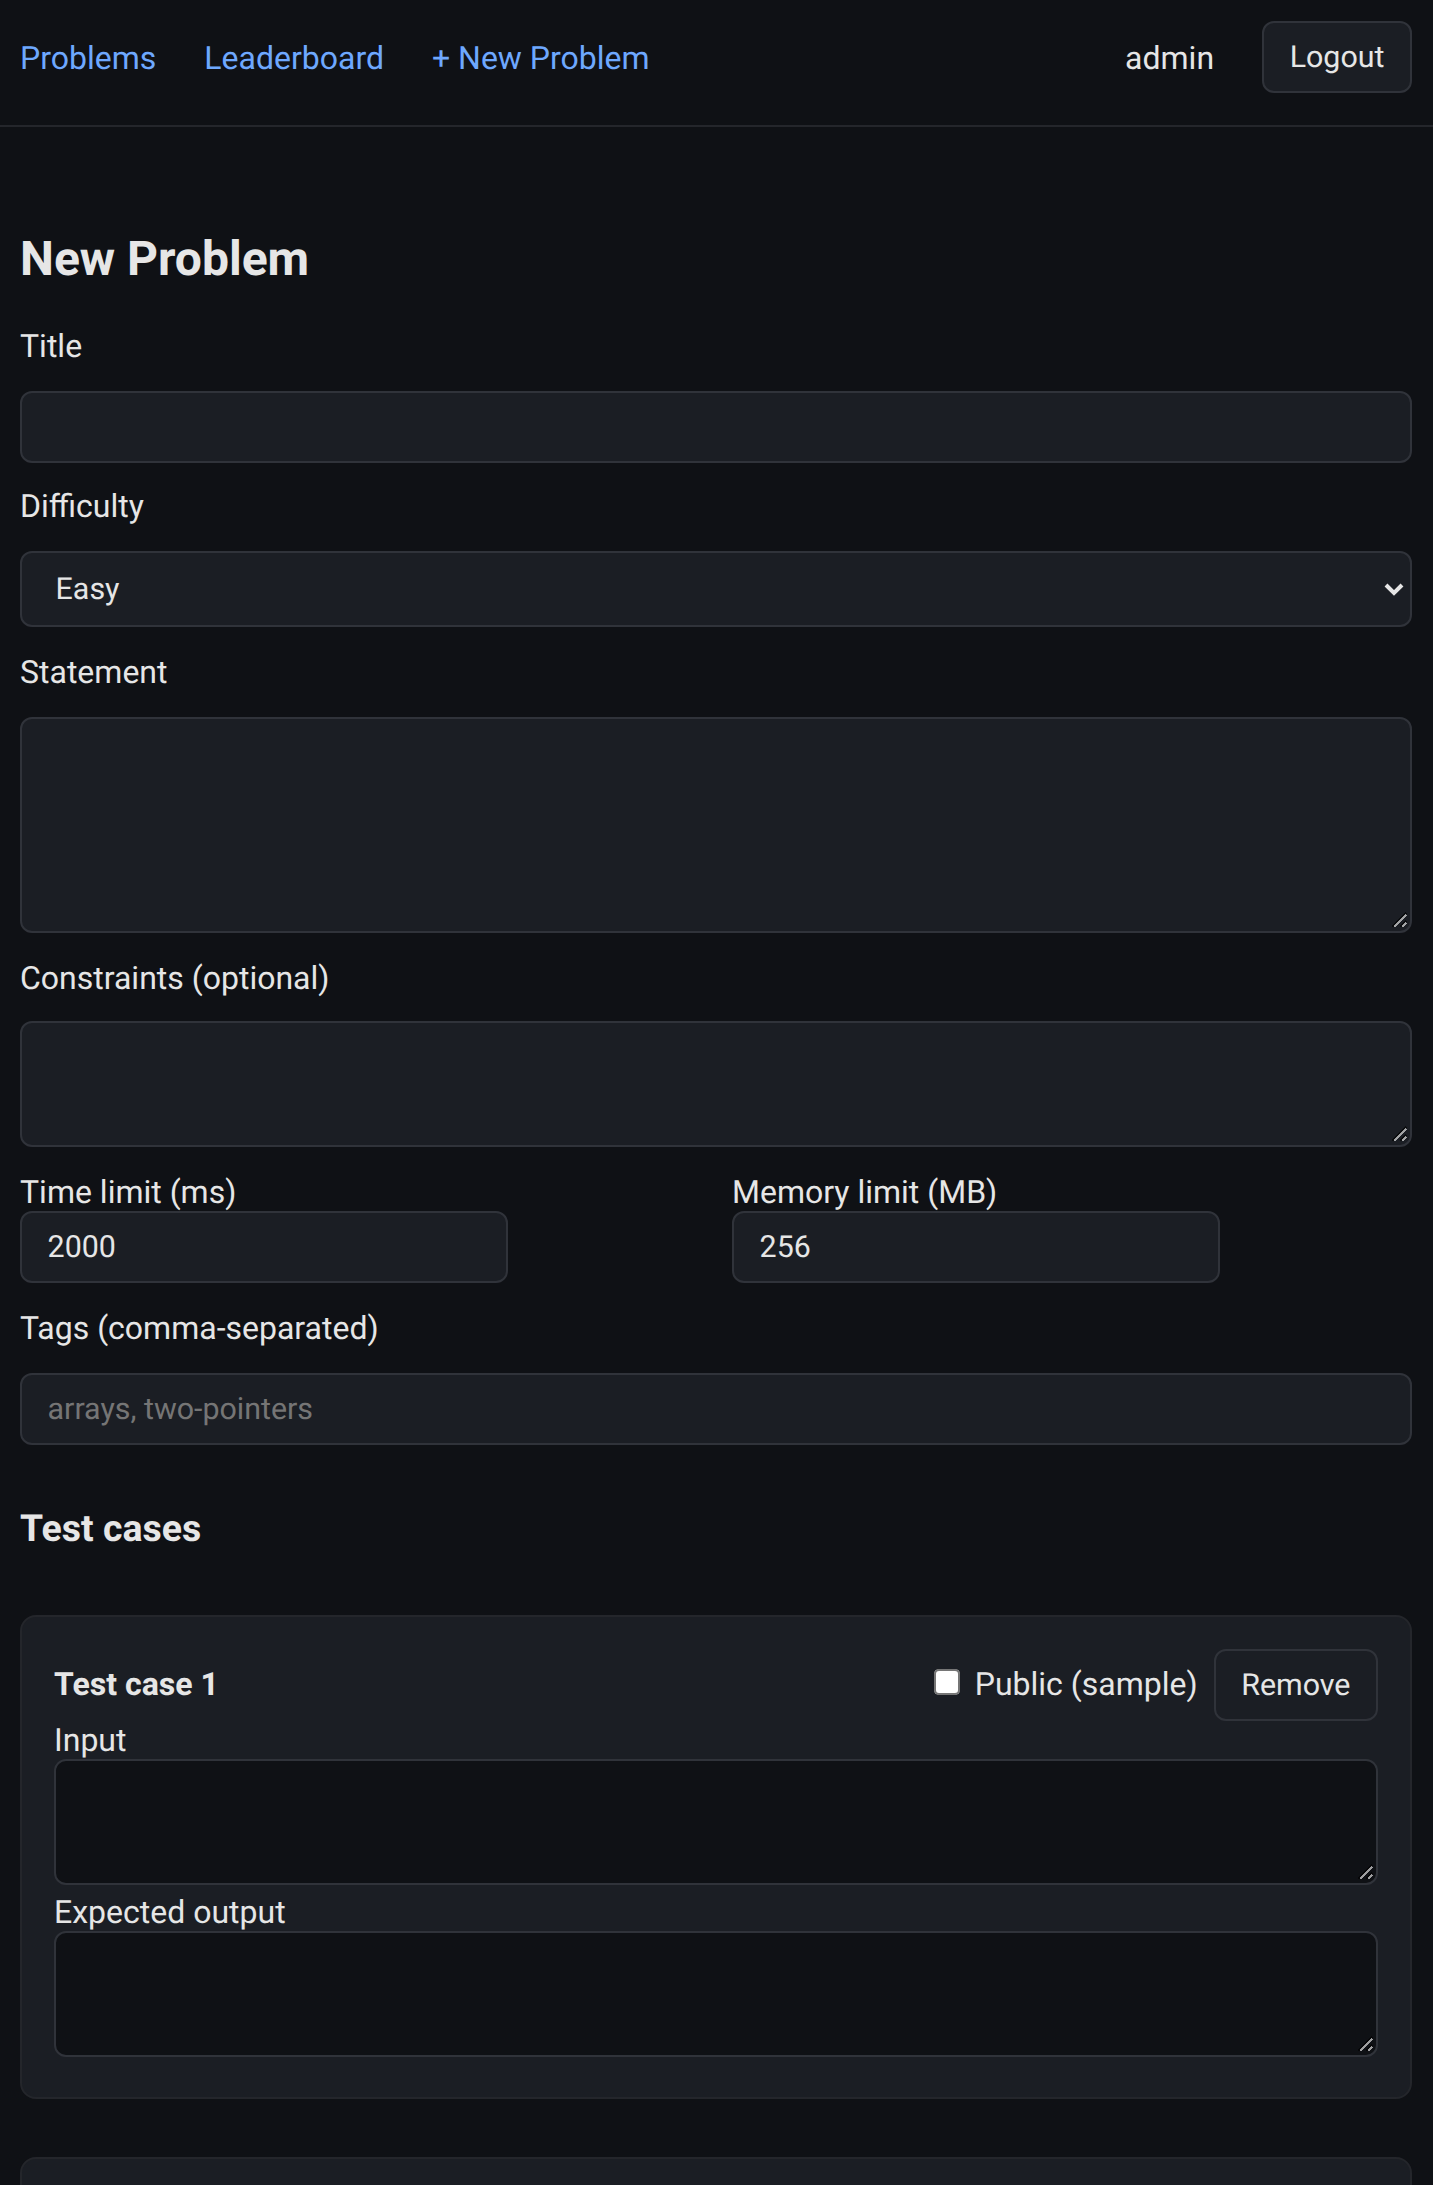
\includegraphics[width=0.85\textwidth]{ui_admin_new_problem.png}
  \caption{The administrator page for creating a new problem, shown through the first test case.}
  \label{fig:adminnew}
\end{figure}

\begin{figure}[htbp]
  \centering
  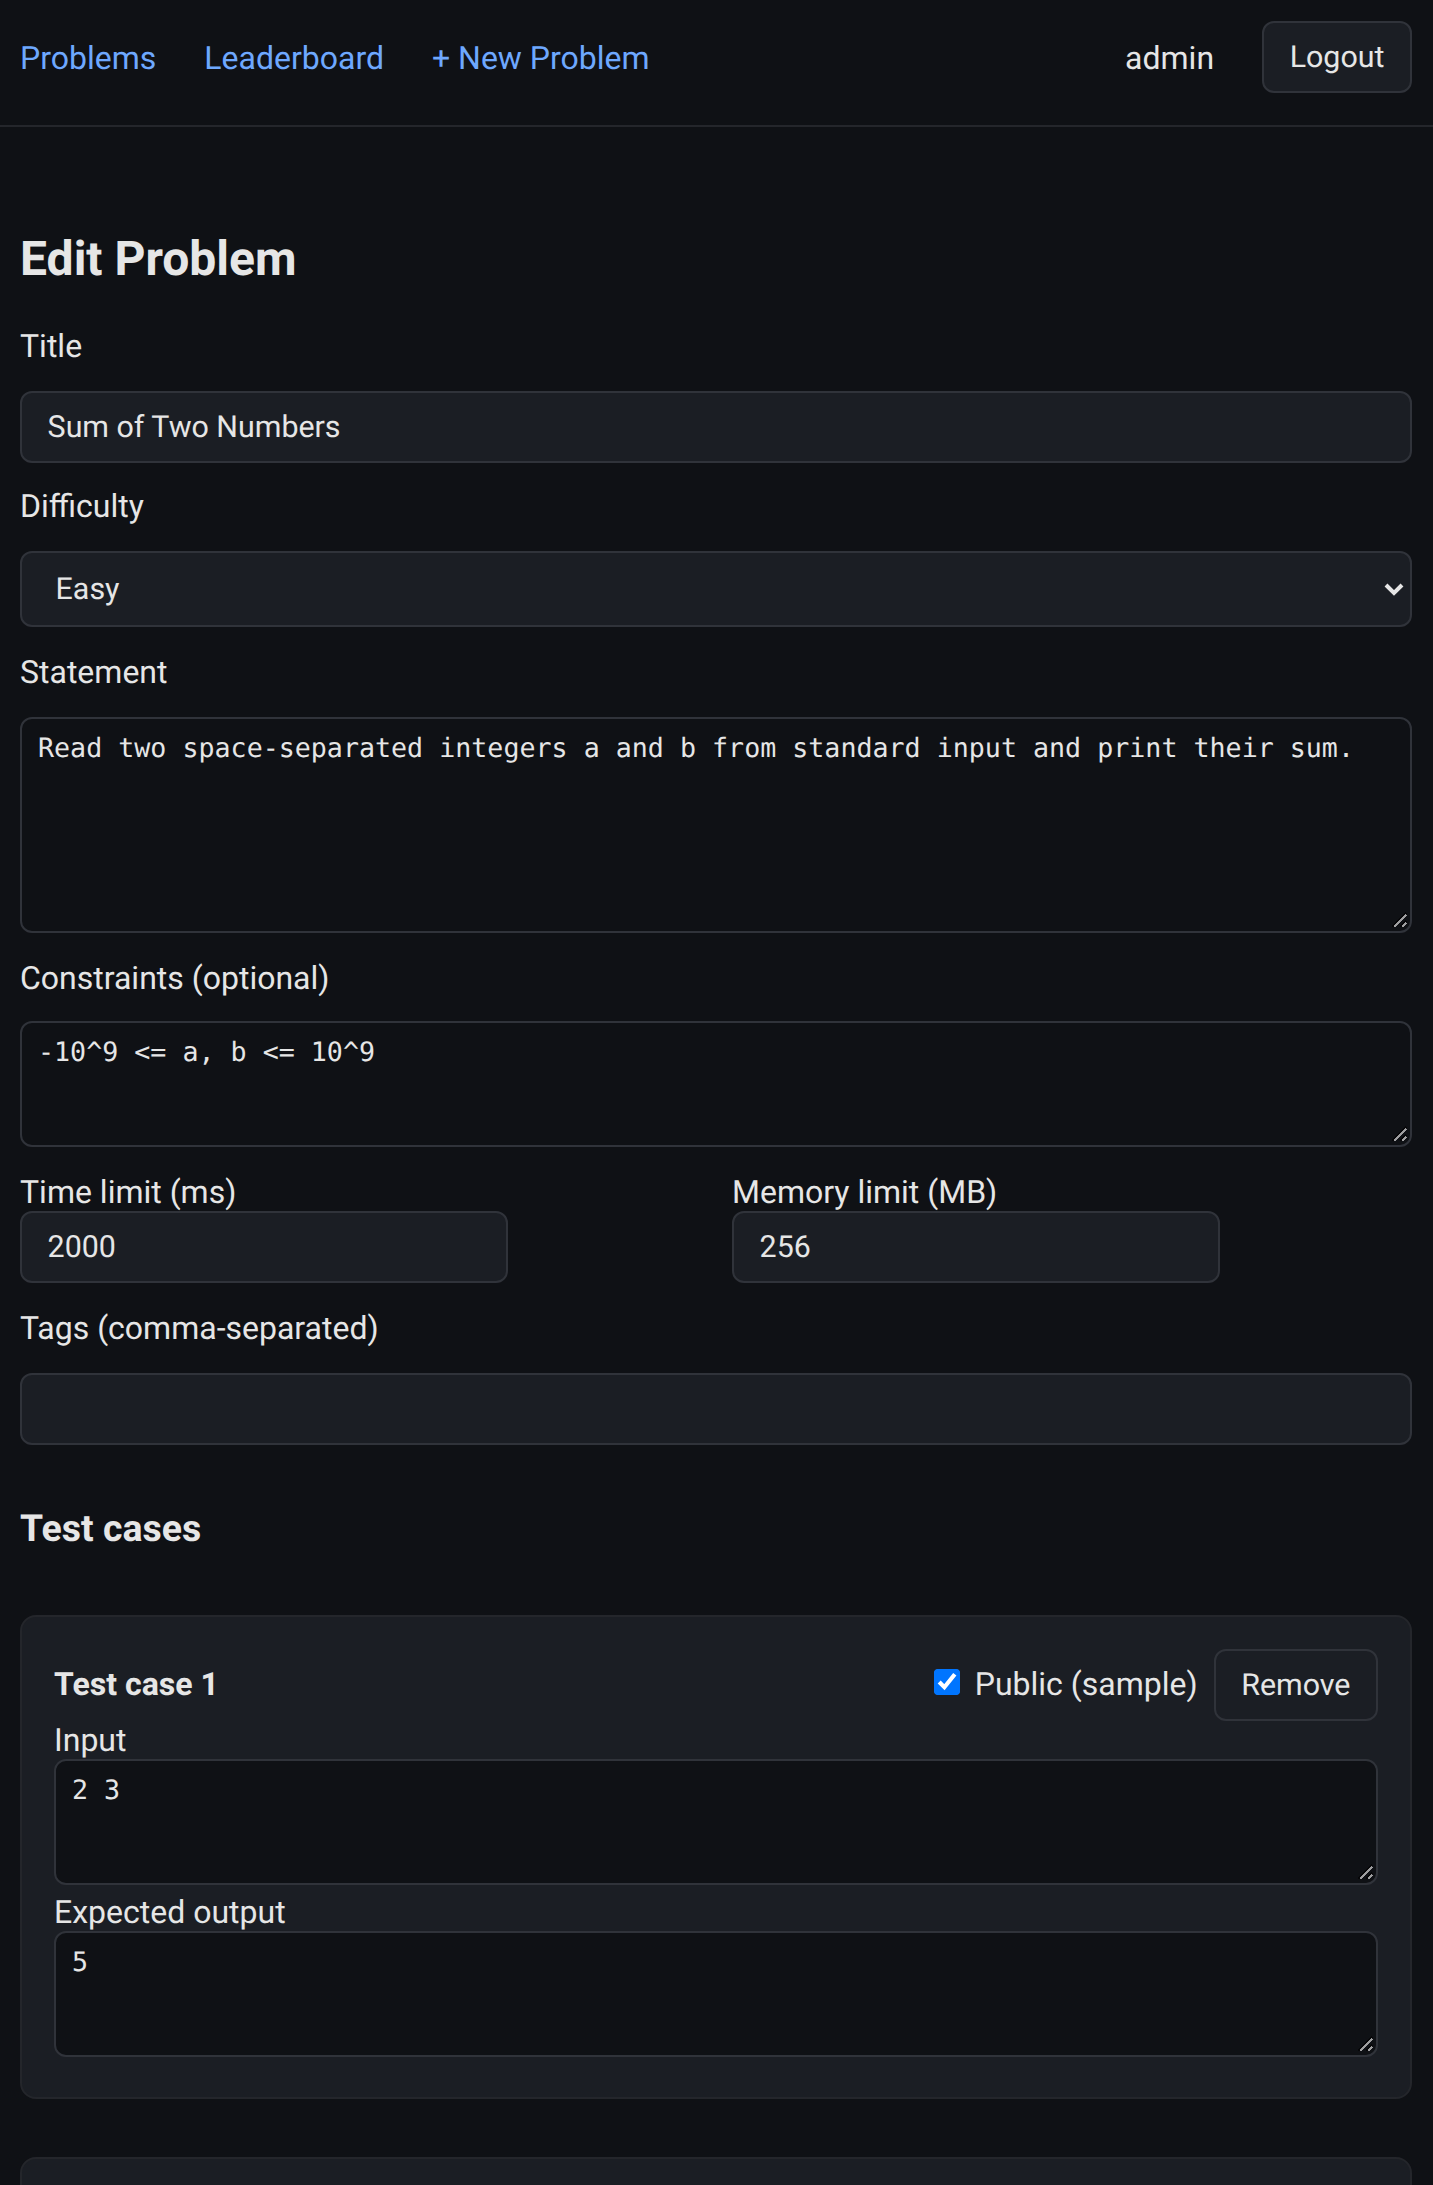
\includegraphics[width=0.85\textwidth]{ui_admin_edit_problem.png}
  \caption{The administrator page for editing an existing problem, shown through the first test case.}
  \label{fig:adminedit}
\end{figure}

\section*{Containerisation and Deployment}
To make the platform easy to run and deploy, every part of it was containerised and wired together with Docker Compose. A multi stage Dockerfile builds the backend into a single runnable artefact, and a second Dockerfile builds the frontend and serves the resulting static files through nginx, which also proxies API requests to the backend. The Compose file brings up four services, namely the frontend, the backend, PostgreSQL and Redis, and starts them in the correct order using a health check on the database.

The backend container is given access to the host Docker daemon so that it can launch sandbox containers, and the judge workspace directory is shared between the backend and the daemon so that the files written for a submission are visible inside its sandbox. This use of the host Docker socket is convenient for a single host deployment but is understood to be a significant privilege, since a container with access to the host Docker socket can effectively control the host; the recommendations chapter discusses safer alternatives for a production setting. The overall deployment topology is shown in Figure~\ref{fig:deployment}.

\begin{figure}[htbp]
  \centering
  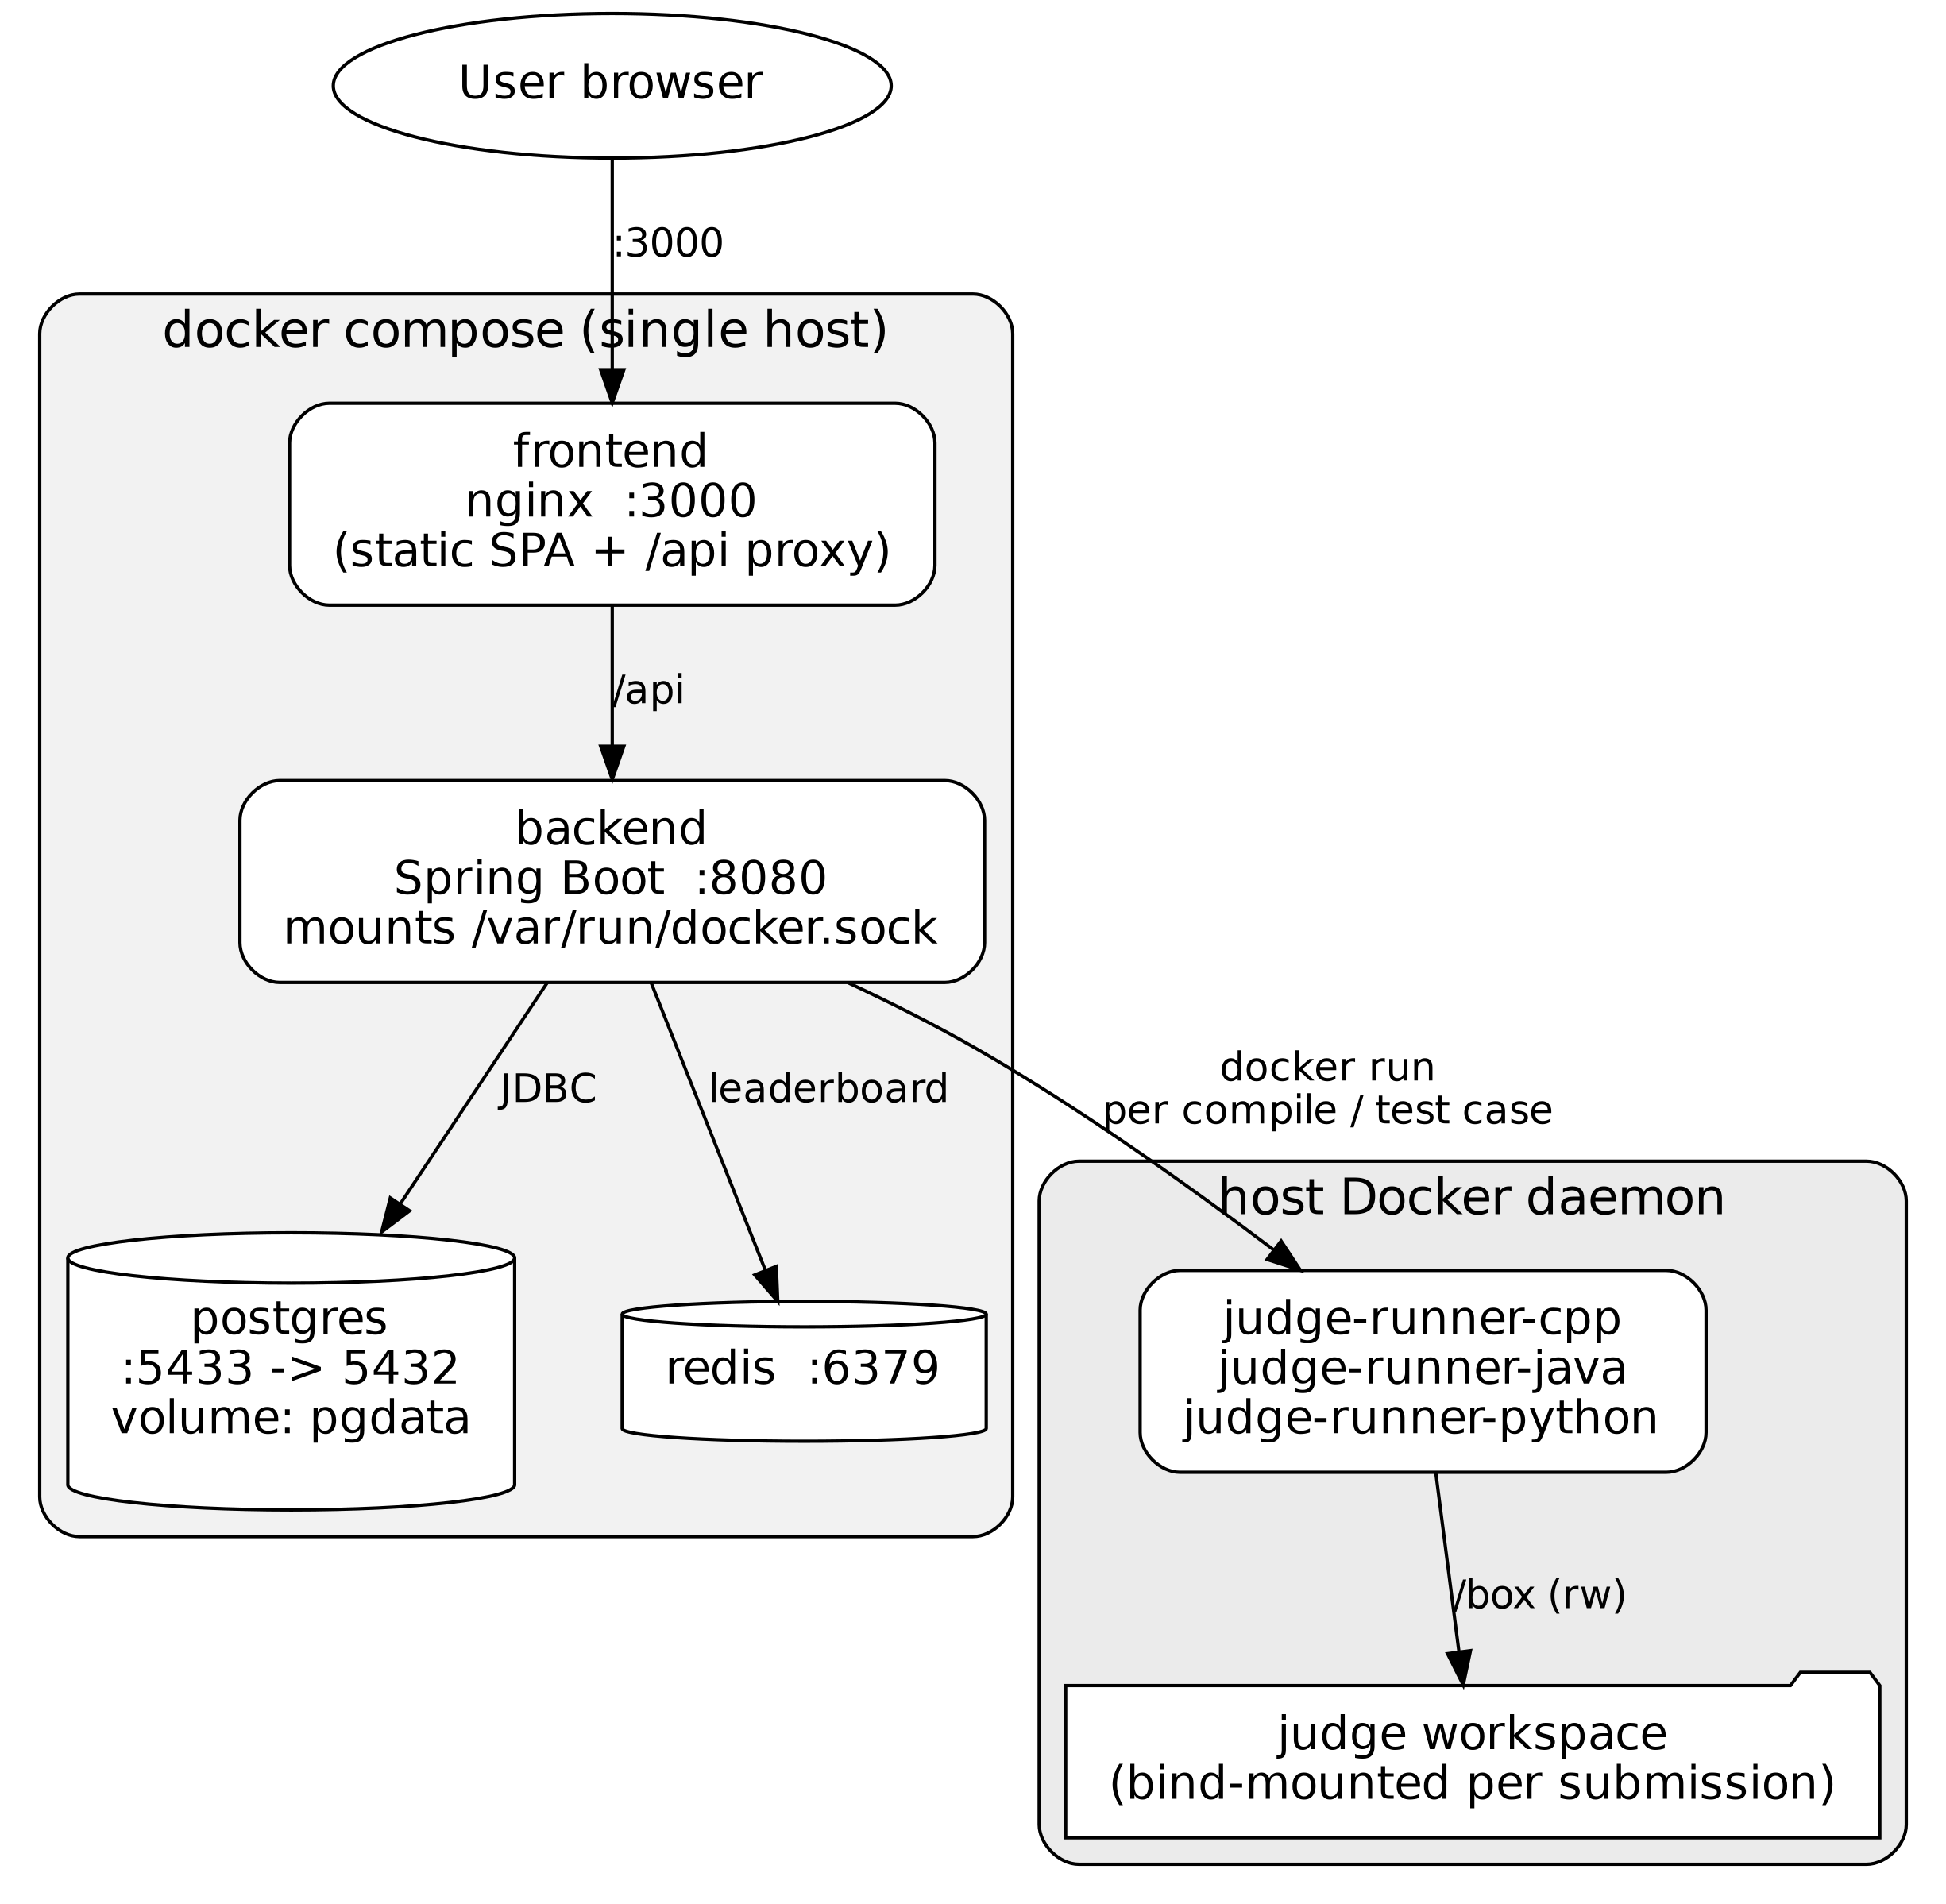
\includegraphics[width=\textwidth]{deployment.png}
  \caption{Docker Compose deployment topology, showing the four services and the sandbox containers launched on the host Docker daemon.}
  \label{fig:deployment}
\end{figure}

\section*{Testing and Validation}
The platform was validated at several levels. Automated unit tests were written for the pure logic that is easy to get wrong, namely the output comparison, with its handling of trailing whitespace, trailing newlines and differing line endings, and the mapping from a container run to a verdict, covering timeouts, out of memory kills, output floods and runtime errors. The judging flow itself was made testable by placing the container execution behind an interface, so that the accepted, wrong answer, time limit exceeded and compile error flows could be exercised with the Docker execution replaced by a mock. A further test confirms that a repeated correct submission for an already solved problem does not increase the leaderboard score, and an integration test running against an in memory database exercises the complete authentication flow of registration, access to a protected endpoint, rejection when unauthenticated, token refresh and login. The full suite passes, as summarised below.

\begin{lstlisting}[caption={Summary of the automated test run.},label={lst:mvn}]
Tests run: 7  -- OutputComparatorTest
Tests run: 6  -- VerdictMappingTest
Tests run: 5  -- JudgeServiceTest
Tests run: 2  -- JudgePersistenceFirstSolveTest
Tests run: 3  -- LeaderboardServiceTest
Tests run: 3  -- AuthIntegrationTest
Tests run: 26, Failures: 0, Errors: 0, Skipped: 0
BUILD SUCCESS
\end{lstlisting}

In addition to the automated tests, an end to end smoke test script was written to drive the whole system through its public API. For a single problem it submits, in each of the three languages, a correct solution, a wrong answer, an infinite loop, a program with a compile error and one that fails at runtime, and it then polls each submission to its final verdict and checks that the verdict is correct. The same script also verifies that a second submission made too quickly is rejected and that the leaderboard reflects the solved problems. Table~\ref{tab:smoke} shows the verdicts obtained for each language and scenario when the script was run against the running system; every case produced the expected verdict and all twenty two checks passed.

\begin{table}[htbp]
  \centering
  \caption{Verdicts obtained by the end to end smoke test across the three languages.
  Verdicts are abbreviated: AC = Accepted, WA = Wrong Answer, TLE = Time Limit Exceeded,
  CE = Compile Error, RE = Runtime Error.}
  \label{tab:smoke}
  \begin{tabular}{|l|c|c|c|}
    \hline
    \textbf{Scenario} & \textbf{C++} & \textbf{Python} & \textbf{Java} \\
    \hline
    Correct solution & AC  & AC  & AC  \\
    \hline
    Wrong answer     & WA  & WA  & WA  \\
    \hline
    Infinite loop    & TLE & TLE & TLE \\
    \hline
    Compile error    & CE  & CE  & CE  \\
    \hline
    Runtime error    & RE  & RE  & RE  \\
    \hline
  \end{tabular}
\end{table}

\chapter*{Learning and Skill Development}
\addcontentsline{toc}{chapter}{Learning and Skill Development}

This internship gave me the opportunity to take a project from an idea to a working, tested system, and the learning that came from that was considerable. On the backend side, I became comfortable with Spring Boot as a framework rather than just as a collection of annotations. I learned how inversion of control and dependency injection shape the way an application is structured, how to design a clean separation between controllers, services and repositories, and how Spring Data JPA maps an object model onto a relational database. Working through entity relationships, pagination and transactions on a real schema made these ideas concrete in a way that reading about them had not.

A large part of my learning was about security and the care that untrusted input demands. Implementing JSON Web Token authentication taught me how stateless authentication actually works, why access and refresh tokens are separated and how a filter integrates with the Spring Security context on each request. More broadly, building a system that runs code written by strangers made me think seriously about isolation and resource control, and I gained a practical understanding of how Docker's networking, memory, process and filesystem controls can be combined to contain a hostile program.

I also learned a great deal about writing software that behaves well under failure and load, rather than only on the happy path. The transaction problem in the judge was a turning point for me, because it showed how a design that works perfectly in a demonstration can still be fundamentally unscalable, and how understanding the way a framework actually implements a feature, in this case the proxy behind transactional methods, is essential to fixing such problems correctly. Learning to reason about timeouts, cleanup of containers and workspaces, and graceful degradation when a dependency like Redis is unavailable, changed the way I think about building reliable systems.

Finally, I improved a range of supporting skills that are part of real software engineering. I became more fluent with Docker and Docker Compose, with building a React frontend and integrating it with a backend API, and with writing automated tests at both the unit and integration level, including the practice of designing code so that it can be tested by substituting a mock for an external dependency. I also practised writing clear documentation and explaining design decisions, which helped me understand my own work more deeply. Together these skills have given me a much stronger sense of how the concepts from my academic study fit together in a complete application.

\chapter*{Challenges Faced}
\addcontentsline{toc}{chapter}{Challenges Faced}

The most persistent challenge throughout the project was running untrusted code safely. It was not difficult to make a program run inside a container, but making sure that no submission could harm the host or interfere with another submission required careful thought about every resource a program might abuse, including the network, memory, the number of processes, the filesystem and the amount of output produced. I had to understand each isolation and resource control option and reason about what would happen if a submission tried to defeat it, and this took several iterations before I was satisfied that the sandbox was tight. Closely related to this was my growing awareness of the risk of giving the backend access to the host Docker socket, which is convenient but effectively hands control of the host to that container, and which I came to understand as a deliberate trade off rather than a free convenience.

A particularly instructive challenge was the long running database transaction in the judge. My first version wrapped the entire asynchronous judging routine in a single transaction, and although it worked, I realised that it held a database connection open across every slow container invocation, which would exhaust the connection pool under load. Fixing this correctly was harder than it looked, because when I first moved the database writes into separate transactional methods they did not actually run in their own transactions. I eventually traced this to the way Spring implements transactions through a proxy, which a call from one method of a class to another method of the same class bypasses. Understanding this self invocation behaviour and restructuring the judge so that the database work lived in a separate component was one of the most valuable lessons of the internship.

Getting the verdicts exactly right was another challenge, because several failure modes can look similar from the outside. Distinguishing a genuine runtime error from a program that was killed for exceeding its memory limit required me to understand how an out of memory kill is reported, and ensuring that a program producing endless output was classified as an output limit problem rather than being allowed to exhaust memory required draining the output on separate threads and capping it. I also had to make sure that a timed out container was actually killed and removed rather than being left running, which I checked by inspecting the list of containers after deliberately submitting an infinite loop.

I also met a number of smaller but time consuming problems that are typical of real development. One that stood out involved the database schema generated automatically from the entity model: when I added a new verdict value, an existing database rejected it because the check constraint created earlier did not include the new value, which taught me the limits of relying on automatic schema updates and why versioned migrations are preferable. Setting up the execution environment also required care, since the way container file sharing works depends on how the Docker daemon is installed, and the judge workspace had to be placed where the daemon could actually see it.

Each of these challenges required me to slow down, read more deeply about how the underlying tools and frameworks behave and test my assumptions directly rather than trusting that something worked because it appeared to. Working through them improved both my technical understanding and my approach to debugging, and they are among the parts of the internship from which I learned the most.

\chapter*{Impact Assessment}
\addcontentsline{toc}{chapter}{Impact Assessment}

The internship had a clear impact on my own development as an engineer. Over the course of the project I moved from studying frameworks in isolation to using them together to build a complete, working system, and in doing so I gained practical confidence in backend development with Spring Boot, in security and authentication, in containerisation and in frontend development. More importantly, I developed a way of thinking about reliability, scalability and safety that I did not have before, learning to ask how a design behaves under load, how it fails and how it contains untrusted input, rather than only whether it works in a demonstration.

For the organisation, the work produced a complete and documented competitive programming platform that can serve as a demonstration of a non trivial full stack system and as a reference implementation for several commonly needed patterns. The project shows a working example of secure stateless authentication, of safely executing untrusted code inside resource limited containers, of keeping database transactions short around slow external work, and of using a cache with a reliable fallback. Because the judging logic is kept self contained and the whole system is tested and packaged with Docker Compose, it can be run and extended easily, which makes it useful as a basis for future work or as teaching material for later interns.

The platform was validated against its objectives in a tangible way. The automated test suite passes in full, and the end to end smoke test confirmed that correct, wrong, non terminating, non compiling and failing submissions all receive the correct verdict in each of the three supported languages, that the rate limit is enforced and that the leaderboard reflects solved problems. This gives confidence that the system behaves as intended and that the design decisions described in this report hold up in practice.

\chapter*{Conclusion}
\addcontentsline{toc}{chapter}{Conclusion}

The internship resulted in a complete competitive programming platform built from the ground up, covering the frontend, the backend, the database and the execution environment. Starting from a focused learning phase on Java, Spring Boot, persistence, security and Docker, the work progressed through system design, authentication, problem management, the judge engine, asynchronous processing, the leaderboard, the frontend and containerisation, and finished with automated testing and documentation. The result is a system in which a user can register, browse problems, submit a solution in C++, Java or Python and receive an automatically determined verdict, with the whole flow working end to end.

The core of the project was the judge engine, and it was here that the most important engineering decisions were made. Running untrusted code safely was achieved by executing every compile step and every test case in a fresh Docker container with network access removed, strict memory, CPU and process limits, a read only filesystem and an unprivileged user, and by capturing output under a bounded cap. Making the judging robust required killing and removing timed out containers, cleaning up workspaces, keeping database transactions short around the slow container work and moving any unexpected failure into a terminal error state rather than leaving a submission stuck.

Beyond the judge, the project applied a number of sound engineering patterns: stateless authentication with separate access and refresh tokens, role based access control, a Redis sorted set used as a cache over an authoritative PostgreSQL store with a graceful fallback, per user rate limiting, consistent error handling and input validation. The system was validated both by an automated test suite, which passes in full, and by an end to end smoke test that confirmed correct behaviour across all three languages and all the main verdicts.

Overall, the internship met its objectives and produced a working, tested and documented platform. Just as importantly, it deepened my understanding of how to build software that is secure, reliable and scalable, and gave me direct experience of the kinds of subtle problems that only appear when a system is taken seriously beyond a simple demonstration. The platform also provides a clear foundation for the extensions described in the following chapter.

\chapter*{Recommendations}
\addcontentsline{toc}{chapter}{Recommendations}

While the platform is complete and works end to end, there are several directions in which it could be developed further, most of which were identified during the project and deliberately left as future work.

The first recommendation concerns scaling the judge. At present a submission is judged in process using asynchronous execution, which is ideal for a single instance but does not allow judging capacity to be scaled independently. Introducing a message queue such as Kafka between the submission step and the judge would allow several judge workers to process submissions in parallel and would provide natural backpressure and durability, and the existing boundary between submitting and judging is a clean place to insert such a queue.

A second recommendation is to replace the polling on the submission page with a push based mechanism such as server sent events or WebSockets. Polling is simple and perfectly adequate for the current scale, but a push based approach would deliver verdicts to the user as soon as they are ready and would remove the repeated requests that polling generates. A related efficiency improvement would be to run all of a submission's test cases inside a single container rather than starting a new container for each test case, which would reduce the per test startup overhead when the number of test cases is large.

The most important recommendation for a production setting concerns the execution environment. The backend currently launches sandboxes through the host Docker socket, which is effectively equivalent to host level privileges and is therefore only suitable for a trusted single host. For a real deployment the sandboxing should be hardened, for example by using a stronger isolation layer such as gVisor or a purpose built sandbox such as nsjail, or by moving judging onto dedicated judge machines that are isolated from the rest of the system. It is also recommended that the database schema be managed with versioned migrations using a tool such as Flyway rather than relying on automatic schema generation, so that changes such as new verdict values can be applied safely to an existing database, and that the per user rate limit be moved into Redis so that it is shared correctly across multiple instances.

\section*{Mode of Working and Ethical Practices}

\textbf{Have you worked in a team or independently?} The internship was carried out independently, with the project designed and implemented by me under the guidance of the industry mentor and the internal faculty mentor. As the work was individual, a team size is not applicable.

\textbf{Have you followed ethical practices?} Ethical practices were followed throughout the project. User passwords are never stored in plain text but only as BCrypt hashes, and sensitive configuration such as the token signing secret and the database password is read from environment variables rather than being hard coded into the source. The platform is built specifically to isolate and contain untrusted user code so that it cannot harm the host or other users, which is itself an ethical as well as a technical requirement. The work is my own, and the open source frameworks and libraries used, such as Spring Boot, React and others, are standard, openly licensed tools that are properly credited in the references.

\chapter*{Acknowledgements}
\addcontentsline{toc}{chapter}{Acknowledgements}

I would like to express my sincere thanks to my external mentor, Neela Santhosh Kumar, Human Resources \& Academic Head at CodTech IT Solutions Pvt.\ Ltd., for giving me the opportunity to work on this project and for the guidance provided on the requirements and direction of the work throughout the internship.

I am grateful to CodTech IT Solutions Pvt.\ Ltd.\ for providing a well structured internship programme and the opportunity to work on a complete and meaningful software engineering project.

I would also like to express my gratitude to my internal mentor, Dr.\ Pratiksha Deshmukh, for the guidance and support provided during the internship, and to COEP Technological University for permitting me to undertake this internship as part of the curriculum and for providing the opportunity to gain practical experience in software development.

Lastly, I would like to thank my family for their constant support and encouragement during the course of this internship.

\chapter*{References}
\addcontentsline{toc}{chapter}{References}

\begin{enumerate}
    \item Spring Boot Reference Documentation, available on the Spring project website.
    \item Spring Security Reference Documentation, available on the Spring project website.
    \item Spring Data JPA Reference Documentation, available on the Spring project website.
    \item Docker Documentation, including the \texttt{docker run} reference and the guide to runtime resource constraints, available at docs.docker.com.
    \item Redis Documentation, Sorted Sets and the ZINCRBY and ZREVRANGE commands, available at redis.io.
    \item React Documentation, available at react.dev.
    \item Vite Documentation, available at vitejs.dev.
    \item Monaco Editor Documentation, available at microsoft.github.io/monaco-editor.
    \item PostgreSQL Documentation, available at postgresql.org.
    \item M.\ Jones, J.\ Bradley and N.\ Sakimura, JSON Web Token (JWT), RFC 7519, Internet Engineering Task Force.
    \item Source code and documentation of the project, including the README and the evaluation notes prepared during the internship.
\end{enumerate}

\end{document}
